\documentclass[a4paper]{book}
\usepackage{makeidx}
\usepackage{graphicx}
\usepackage{multicol}
\usepackage{float}
\usepackage{listings}
\usepackage{color}
\usepackage{textcomp}
\usepackage{alltt}
\usepackage{times}
\usepackage{ifpdf}
\ifpdf
\usepackage[pdftex,
            pagebackref=true,
            colorlinks=true,
            linkcolor=blue,
            unicode
           ]{hyperref}
\else
\usepackage[ps2pdf,
            pagebackref=true,
            colorlinks=true,
            linkcolor=blue,
            unicode
           ]{hyperref}
\usepackage{pspicture}
\fi
\usepackage[utf8]{inputenc}
\usepackage{doxygen}
\lstset{language=C++,inputencoding=utf8,basicstyle=\footnotesize,breaklines=true,breakatwhitespace=true,tabsize=8,numbers=left }
\makeindex
\setcounter{tocdepth}{3}
\renewcommand{\footrulewidth}{0.4pt}
\begin{document}
\hypersetup{pageanchor=false}
\begin{titlepage}
\vspace*{7cm}
\begin{center}
{\Large GDL-\/GL \\[1ex]\large 1.1 }\\
\vspace*{1cm}
{\large Generated by Doxygen 1.6.2-20100208}\\
\vspace*{0.5cm}
{\small Mon May 16 20:00:43 2011}\\
\end{center}
\end{titlepage}
\clearemptydoublepage
\pagenumbering{roman}
\tableofcontents
\clearemptydoublepage
\pagenumbering{arabic}
\hypersetup{pageanchor=true}
\chapter{Class Index}
\section{Class Hierarchy}
This inheritance list is sorted roughly, but not completely, alphabetically:\begin{DoxyCompactList}
\item \contentsline{section}{gdl::Color}{\pageref{structgdl_1_1Color}}{}
\item \contentsline{section}{gdl::Game}{\pageref{classgdl_1_1Game}}{}
\item \contentsline{section}{gdl::IClock}{\pageref{classgdl_1_1IClock}}{}
\begin{DoxyCompactList}
\item \contentsline{section}{gdl::Clock}{\pageref{classgdl_1_1Clock}}{}
\item \contentsline{section}{gdl::GameClock}{\pageref{classgdl_1_1GameClock}}{}
\end{DoxyCompactList}
\item \contentsline{section}{gdl::Input}{\pageref{classgdl_1_1Input}}{}
\item \contentsline{section}{gdl::ModelException}{\pageref{classgdl_1_1ModelException}}{}
\item \contentsline{section}{gdl::ResourceBase}{\pageref{classgdl_1_1ResourceBase}}{}
\begin{DoxyCompactList}
\item \contentsline{section}{gdl::Resource$<$ Type $>$}{\pageref{classgdl_1_1Resource}}{}
\item \contentsline{section}{gdl::Resource$<$ ImageImpl $>$}{\pageref{classgdl_1_1Resource}}{}
\begin{DoxyCompactList}
\item \contentsline{section}{gdl::Image}{\pageref{classgdl_1_1Image}}{}
\end{DoxyCompactList}
\item \contentsline{section}{gdl::Resource$<$ ModelImpl $>$}{\pageref{classgdl_1_1Resource}}{}
\begin{DoxyCompactList}
\item \contentsline{section}{gdl::Model}{\pageref{classgdl_1_1Model}}{}
\end{DoxyCompactList}
\end{DoxyCompactList}
\item \contentsline{section}{gdl::Window}{\pageref{classgdl_1_1Window}}{}
\end{DoxyCompactList}

\chapter{Class Index}
\section{Class List}
Here are the classes, structs, unions and interfaces with brief descriptions:\begin{DoxyCompactList}
\item\contentsline{section}{\hyperlink{classgdl_1_1Clock}{gdl::Clock} }{\pageref{classgdl_1_1Clock}}{}
\item\contentsline{section}{\hyperlink{structgdl_1_1Color}{gdl::Color} }{\pageref{structgdl_1_1Color}}{}
\item\contentsline{section}{\hyperlink{classgdl_1_1Game}{gdl::Game} }{\pageref{classgdl_1_1Game}}{}
\item\contentsline{section}{\hyperlink{classgdl_1_1GameClock}{gdl::GameClock} }{\pageref{classgdl_1_1GameClock}}{}
\item\contentsline{section}{\hyperlink{classgdl_1_1IClock}{gdl::IClock} }{\pageref{classgdl_1_1IClock}}{}
\item\contentsline{section}{\hyperlink{classgdl_1_1Image}{gdl::Image} }{\pageref{classgdl_1_1Image}}{}
\item\contentsline{section}{\hyperlink{classgdl_1_1Input}{gdl::Input} }{\pageref{classgdl_1_1Input}}{}
\item\contentsline{section}{\hyperlink{classgdl_1_1Model}{gdl::Model} }{\pageref{classgdl_1_1Model}}{}
\item\contentsline{section}{\hyperlink{classgdl_1_1ModelException}{gdl::ModelException} }{\pageref{classgdl_1_1ModelException}}{}
\item\contentsline{section}{\hyperlink{classgdl_1_1Resource}{gdl::Resource$<$ Type $>$} }{\pageref{classgdl_1_1Resource}}{}
\item\contentsline{section}{\hyperlink{classgdl_1_1ResourceBase}{gdl::ResourceBase} }{\pageref{classgdl_1_1ResourceBase}}{}
\item\contentsline{section}{\hyperlink{classgdl_1_1Window}{gdl::Window} }{\pageref{classgdl_1_1Window}}{}
\end{DoxyCompactList}

\chapter{Class Documentation}
\hypertarget{classgdl_1_1Clock}{
\section{gdl::Clock Class Reference}
\label{classgdl_1_1Clock}\index{gdl::Clock@{gdl::Clock}}
}


{\ttfamily \#include $<$Clock.hpp$>$}Inheritance diagram for gdl::Clock::\begin{figure}[H]
\begin{center}
\leavevmode
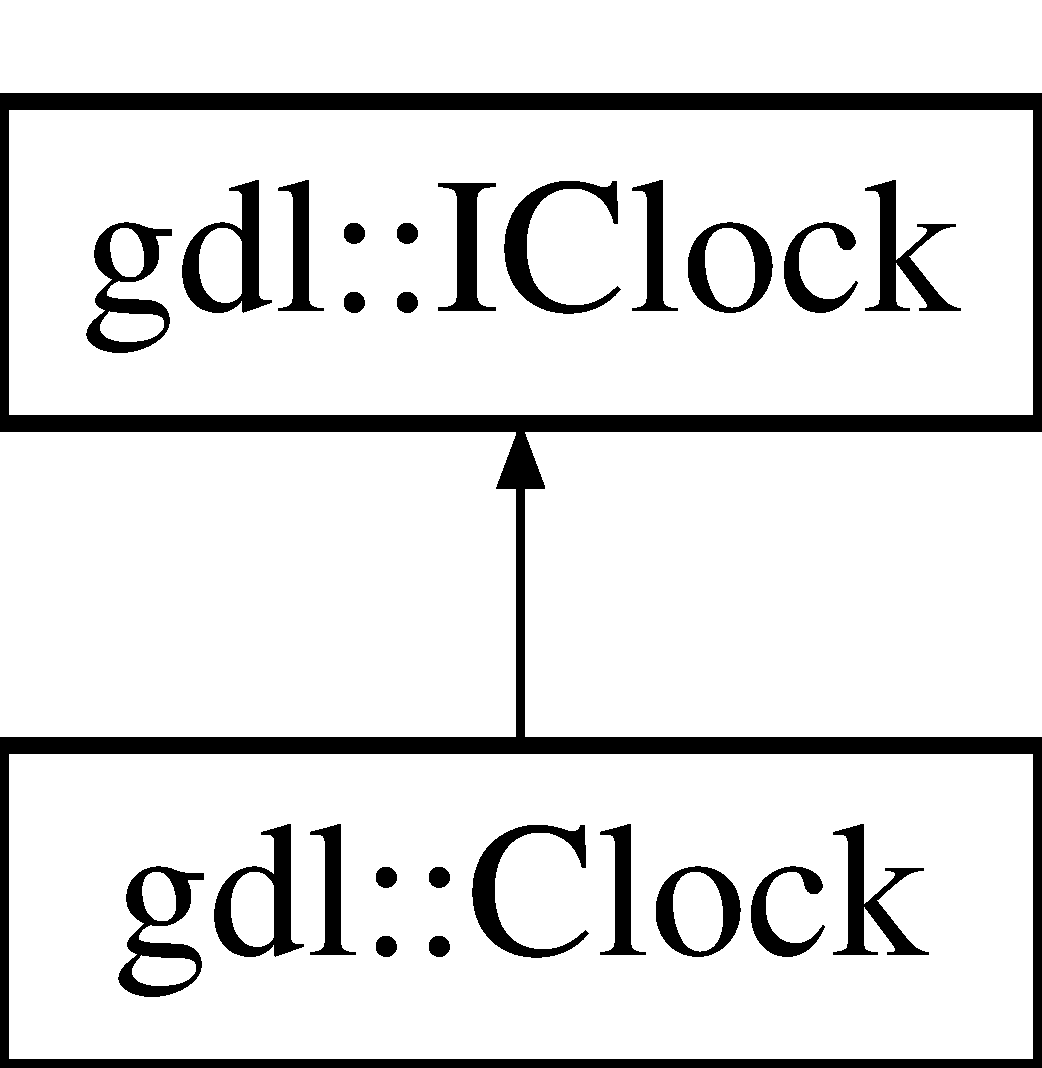
\includegraphics[height=2cm]{classgdl_1_1Clock}
\end{center}
\end{figure}
\subsection*{Public Member Functions}
\begin{DoxyCompactItemize}
\item 
\hyperlink{classgdl_1_1Clock_aab3b54f0e335efd7136e8a2900da9c3e}{Clock} ()
\item 
\hyperlink{classgdl_1_1Clock_a54c8e0862b5903056d169195c0b22072}{$\sim$Clock} ()
\item 
void \hyperlink{classgdl_1_1Clock_af1054a354823d2556a780ddec710e368}{play} (void)
\item 
void \hyperlink{classgdl_1_1Clock_afcd4590e0217065f7f2c9bd13cb6c3ad}{pause} (void)
\item 
void \hyperlink{classgdl_1_1Clock_acc748cbe2dc79ab94c7843e2f010d049}{update} (void)
\item 
void \hyperlink{classgdl_1_1Clock_a9a44b0217d50c216d2e94d0f174e3a67}{reset} (void)
\item 
float \hyperlink{classgdl_1_1Clock_a3b81a05f6b9d4af46b6c955017c8ddfd}{getElapsedTime} (void) const 
\item 
float \hyperlink{classgdl_1_1Clock_a1c7cb8d2c1c742db97cb667c2cfe5552}{getTotalElapsedTime} (void) const 
\end{DoxyCompactItemize}


\subsection{Detailed Description}
\hyperlink{classgdl_1_1Clock}{Clock} is used to force a specific time implementation. 

\subsection{Constructor \& Destructor Documentation}
\hypertarget{classgdl_1_1Clock_aab3b54f0e335efd7136e8a2900da9c3e}{
\index{gdl::Clock@{gdl::Clock}!Clock@{Clock}}
\index{Clock@{Clock}!gdl::Clock@{gdl::Clock}}
\subsubsection[{Clock}]{\setlength{\rightskip}{0pt plus 5cm}gdl::Clock::Clock ()}}
\label{classgdl_1_1Clock_aab3b54f0e335efd7136e8a2900da9c3e}
Default constructror. \hypertarget{classgdl_1_1Clock_a54c8e0862b5903056d169195c0b22072}{
\index{gdl::Clock@{gdl::Clock}!$\sim$Clock@{$\sim$Clock}}
\index{$\sim$Clock@{$\sim$Clock}!gdl::Clock@{gdl::Clock}}
\subsubsection[{$\sim$Clock}]{\setlength{\rightskip}{0pt plus 5cm}gdl::Clock::$\sim$Clock ()}}
\label{classgdl_1_1Clock_a54c8e0862b5903056d169195c0b22072}
Default destructror. 

\subsection{Member Function Documentation}
\hypertarget{classgdl_1_1Clock_a3b81a05f6b9d4af46b6c955017c8ddfd}{
\index{gdl::Clock@{gdl::Clock}!getElapsedTime@{getElapsedTime}}
\index{getElapsedTime@{getElapsedTime}!gdl::Clock@{gdl::Clock}}
\subsubsection[{getElapsedTime}]{\setlength{\rightskip}{0pt plus 5cm}float gdl::Clock::getElapsedTime (void) const\hspace{0.3cm}{\ttfamily  \mbox{[}virtual\mbox{]}}}}
\label{classgdl_1_1Clock_a3b81a05f6b9d4af46b6c955017c8ddfd}
Return the time between two call of the update method.

\begin{DoxyReturn}{Returns}
The time in float. 
\end{DoxyReturn}


Implements \hyperlink{classgdl_1_1IClock_ad5c3e51562a10e319a3494785d077d1b}{gdl::IClock}.\hypertarget{classgdl_1_1Clock_a1c7cb8d2c1c742db97cb667c2cfe5552}{
\index{gdl::Clock@{gdl::Clock}!getTotalElapsedTime@{getTotalElapsedTime}}
\index{getTotalElapsedTime@{getTotalElapsedTime}!gdl::Clock@{gdl::Clock}}
\subsubsection[{getTotalElapsedTime}]{\setlength{\rightskip}{0pt plus 5cm}float gdl::Clock::getTotalElapsedTime (void) const}}
\label{classgdl_1_1Clock_a1c7cb8d2c1c742db97cb667c2cfe5552}
Return the time between now and the instantiation of the \hyperlink{classgdl_1_1Game}{Game} class.

\begin{DoxyReturn}{Returns}
The time in float. 
\end{DoxyReturn}
\hypertarget{classgdl_1_1Clock_afcd4590e0217065f7f2c9bd13cb6c3ad}{
\index{gdl::Clock@{gdl::Clock}!pause@{pause}}
\index{pause@{pause}!gdl::Clock@{gdl::Clock}}
\subsubsection[{pause}]{\setlength{\rightskip}{0pt plus 5cm}void gdl::Clock::pause (void)\hspace{0.3cm}{\ttfamily  \mbox{[}virtual\mbox{]}}}}
\label{classgdl_1_1Clock_afcd4590e0217065f7f2c9bd13cb6c3ad}
Pause the clock until you play it again. 

Implements \hyperlink{classgdl_1_1IClock_a7274430efa1f0e621bcce5d99d6abca7}{gdl::IClock}.\hypertarget{classgdl_1_1Clock_af1054a354823d2556a780ddec710e368}{
\index{gdl::Clock@{gdl::Clock}!play@{play}}
\index{play@{play}!gdl::Clock@{gdl::Clock}}
\subsubsection[{play}]{\setlength{\rightskip}{0pt plus 5cm}void gdl::Clock::play (void)\hspace{0.3cm}{\ttfamily  \mbox{[}virtual\mbox{]}}}}
\label{classgdl_1_1Clock_af1054a354823d2556a780ddec710e368}
Start the clock. 

Implements \hyperlink{classgdl_1_1IClock_af9f70e18cd6b9b39aca1a359412adf4d}{gdl::IClock}.\hypertarget{classgdl_1_1Clock_a9a44b0217d50c216d2e94d0f174e3a67}{
\index{gdl::Clock@{gdl::Clock}!reset@{reset}}
\index{reset@{reset}!gdl::Clock@{gdl::Clock}}
\subsubsection[{reset}]{\setlength{\rightskip}{0pt plus 5cm}void gdl::Clock::reset (void)\hspace{0.3cm}{\ttfamily  \mbox{[}virtual\mbox{]}}}}
\label{classgdl_1_1Clock_a9a44b0217d50c216d2e94d0f174e3a67}
Reset the clock to 0. 

Implements \hyperlink{classgdl_1_1IClock_a63cd29fcd9830e719d4cb82d5e993ec6}{gdl::IClock}.\hypertarget{classgdl_1_1Clock_acc748cbe2dc79ab94c7843e2f010d049}{
\index{gdl::Clock@{gdl::Clock}!update@{update}}
\index{update@{update}!gdl::Clock@{gdl::Clock}}
\subsubsection[{update}]{\setlength{\rightskip}{0pt plus 5cm}void gdl::Clock::update (void)\hspace{0.3cm}{\ttfamily  \mbox{[}virtual\mbox{]}}}}
\label{classgdl_1_1Clock_acc748cbe2dc79ab94c7843e2f010d049}
Up the time of the clock. 

Implements \hyperlink{classgdl_1_1IClock_a0489f6f9055df40116e98e7ed6ad4146}{gdl::IClock}.

The documentation for this class was generated from the following files:\begin{DoxyCompactItemize}
\item 
Clock.hpp\item 
Clock.cpp\end{DoxyCompactItemize}

\hypertarget{structgdl_1_1Color}{
\section{gdl::Color Struct Reference}
\label{structgdl_1_1Color}\index{gdl::Color@{gdl::Color}}
}


{\ttfamily \#include $<$Color.hpp$>$}\subsection*{Public Types}
\begin{DoxyCompactItemize}
\item 
typedef unsigned char \hyperlink{structgdl_1_1Color_a5f5cae76580de8bc9abf0ca1ab33e126}{uchar}
\end{DoxyCompactItemize}
\subsection*{Public Member Functions}
\begin{DoxyCompactItemize}
\item 
\hyperlink{structgdl_1_1Color_aa898b04614ee1e721a5413cb9b6cae16}{Color} ()
\item 
\hyperlink{structgdl_1_1Color_a7c67cb8a5174ca1f0817857a6ef37fef}{Color} (\hyperlink{structgdl_1_1Color_a5f5cae76580de8bc9abf0ca1ab33e126}{uchar} \hyperlink{structgdl_1_1Color_aacd5f4d3c04fd4f47986f400a70c9143}{r}, \hyperlink{structgdl_1_1Color_a5f5cae76580de8bc9abf0ca1ab33e126}{uchar} \hyperlink{structgdl_1_1Color_a47b05c3bbf1ece915e3cd7e260b5bfa4}{g}, \hyperlink{structgdl_1_1Color_a5f5cae76580de8bc9abf0ca1ab33e126}{uchar} \hyperlink{structgdl_1_1Color_aa0b3ca9d0a465b76b4bc955ba2c38352}{b}, \hyperlink{structgdl_1_1Color_a5f5cae76580de8bc9abf0ca1ab33e126}{uchar} \hyperlink{structgdl_1_1Color_af3fd2777ff073f3020d5d1fa1d25e38b}{a}=255)
\item 
\hyperlink{structgdl_1_1Color_a416bf40b4967d73bb91023ec8dd56994}{Color} (const \hyperlink{structgdl_1_1Color}{Color} \&)
\item 
\hyperlink{structgdl_1_1Color_afb38b5f4475e657c82c6e0c4e835d1ea}{$\sim$Color} (void)
\item 
\hyperlink{structgdl_1_1Color}{Color} \& \hyperlink{structgdl_1_1Color_a3ef6a664a4ae454eb846ea381c679dba}{operator=} (\hyperlink{structgdl_1_1Color}{Color} const \&)
\item 
bool \hyperlink{structgdl_1_1Color_a90c8f9a5fe3bca45d2760619097f3be2}{operator==} (\hyperlink{structgdl_1_1Color}{Color} const \&) const 
\item 
bool \hyperlink{structgdl_1_1Color_af2fbc33fd8ab45ab40fd61bc1acf67ad}{operator!=} (\hyperlink{structgdl_1_1Color}{Color} const \&) const 
\end{DoxyCompactItemize}
\subsection*{Public Attributes}
\begin{DoxyCompactItemize}
\item 
\hyperlink{structgdl_1_1Color_a5f5cae76580de8bc9abf0ca1ab33e126}{uchar} \hyperlink{structgdl_1_1Color_aacd5f4d3c04fd4f47986f400a70c9143}{r}
\item 
\hyperlink{structgdl_1_1Color_a5f5cae76580de8bc9abf0ca1ab33e126}{uchar} \hyperlink{structgdl_1_1Color_a47b05c3bbf1ece915e3cd7e260b5bfa4}{g}
\item 
\hyperlink{structgdl_1_1Color_a5f5cae76580de8bc9abf0ca1ab33e126}{uchar} \hyperlink{structgdl_1_1Color_aa0b3ca9d0a465b76b4bc955ba2c38352}{b}
\item 
\hyperlink{structgdl_1_1Color_a5f5cae76580de8bc9abf0ca1ab33e126}{uchar} \hyperlink{structgdl_1_1Color_af3fd2777ff073f3020d5d1fa1d25e38b}{a}
\end{DoxyCompactItemize}


\subsection{Detailed Description}
The color class provides an simple container to manage colors. 

\subsection{Member Typedef Documentation}
\hypertarget{structgdl_1_1Color_a5f5cae76580de8bc9abf0ca1ab33e126}{
\index{gdl::Color@{gdl::Color}!uchar@{uchar}}
\index{uchar@{uchar}!gdl::Color@{gdl::Color}}
\subsubsection[{uchar}]{\setlength{\rightskip}{0pt plus 5cm}typedef unsigned char {\bf gdl::Color::uchar}}}
\label{structgdl_1_1Color_a5f5cae76580de8bc9abf0ca1ab33e126}
Type redefinition. 

\subsection{Constructor \& Destructor Documentation}
\hypertarget{structgdl_1_1Color_aa898b04614ee1e721a5413cb9b6cae16}{
\index{gdl::Color@{gdl::Color}!Color@{Color}}
\index{Color@{Color}!gdl::Color@{gdl::Color}}
\subsubsection[{Color}]{\setlength{\rightskip}{0pt plus 5cm}gdl::Color::Color ()}}
\label{structgdl_1_1Color_aa898b04614ee1e721a5413cb9b6cae16}
Default constructor. \hypertarget{structgdl_1_1Color_a7c67cb8a5174ca1f0817857a6ef37fef}{
\index{gdl::Color@{gdl::Color}!Color@{Color}}
\index{Color@{Color}!gdl::Color@{gdl::Color}}
\subsubsection[{Color}]{\setlength{\rightskip}{0pt plus 5cm}gdl::Color::Color ({\bf uchar} {\em r}, \/  {\bf uchar} {\em g}, \/  {\bf uchar} {\em b}, \/  {\bf uchar} {\em a} = {\ttfamily 255})}}
\label{structgdl_1_1Color_a7c67cb8a5174ca1f0817857a6ef37fef}
Constructor.


\begin{DoxyParams}{Parameters}
\item[\mbox{$\leftarrow$} {\em r}]Byte for red component. \item[\mbox{$\leftarrow$} {\em g}]Byte for green component. \item[\mbox{$\leftarrow$} {\em b}]Byte for blue component. \item[\mbox{$\leftarrow$} {\em a}]Byte for alpha component. \end{DoxyParams}
\hypertarget{structgdl_1_1Color_a416bf40b4967d73bb91023ec8dd56994}{
\index{gdl::Color@{gdl::Color}!Color@{Color}}
\index{Color@{Color}!gdl::Color@{gdl::Color}}
\subsubsection[{Color}]{\setlength{\rightskip}{0pt plus 5cm}gdl::Color::Color (const {\bf Color} \& {\em color})}}
\label{structgdl_1_1Color_a416bf40b4967d73bb91023ec8dd56994}
Copy constructor.


\begin{DoxyParams}{Parameters}
\item[\mbox{$\leftarrow$} {\em color}]Instance to copy. \end{DoxyParams}
\hypertarget{structgdl_1_1Color_afb38b5f4475e657c82c6e0c4e835d1ea}{
\index{gdl::Color@{gdl::Color}!$\sim$Color@{$\sim$Color}}
\index{$\sim$Color@{$\sim$Color}!gdl::Color@{gdl::Color}}
\subsubsection[{$\sim$Color}]{\setlength{\rightskip}{0pt plus 5cm}gdl::Color::$\sim$Color (void)\hspace{0.3cm}{\ttfamily  \mbox{[}inline\mbox{]}}}}
\label{structgdl_1_1Color_afb38b5f4475e657c82c6e0c4e835d1ea}
Default destructor. 

\subsection{Member Function Documentation}
\hypertarget{structgdl_1_1Color_af2fbc33fd8ab45ab40fd61bc1acf67ad}{
\index{gdl::Color@{gdl::Color}!operator!=@{operator!=}}
\index{operator!=@{operator!=}!gdl::Color@{gdl::Color}}
\subsubsection[{operator!=}]{\setlength{\rightskip}{0pt plus 5cm}bool gdl::Color::operator!= ({\bf Color} const \& {\em c}) const}}
\label{structgdl_1_1Color_af2fbc33fd8ab45ab40fd61bc1acf67ad}
Overloading of the comparison operator.

\begin{DoxyReturn}{Returns}
If the test succeed, true is returned. Otherwise, false is returned. 
\end{DoxyReturn}
\hypertarget{structgdl_1_1Color_a3ef6a664a4ae454eb846ea381c679dba}{
\index{gdl::Color@{gdl::Color}!operator=@{operator=}}
\index{operator=@{operator=}!gdl::Color@{gdl::Color}}
\subsubsection[{operator=}]{\setlength{\rightskip}{0pt plus 5cm}{\bf Color} \& gdl::Color::operator= ({\bf Color} const \& {\em color})}}
\label{structgdl_1_1Color_a3ef6a664a4ae454eb846ea381c679dba}
Overloading of the assignment operator.

\begin{DoxyReturn}{Returns}
An reference on the \hyperlink{structgdl_1_1Color}{Color} instance. 
\end{DoxyReturn}
\hypertarget{structgdl_1_1Color_a90c8f9a5fe3bca45d2760619097f3be2}{
\index{gdl::Color@{gdl::Color}!operator==@{operator==}}
\index{operator==@{operator==}!gdl::Color@{gdl::Color}}
\subsubsection[{operator==}]{\setlength{\rightskip}{0pt plus 5cm}bool gdl::Color::operator== ({\bf Color} const \& {\em c}) const}}
\label{structgdl_1_1Color_a90c8f9a5fe3bca45d2760619097f3be2}
Overloading of the comparison operator.

\begin{DoxyReturn}{Returns}
If the test succeed, true is returned. Otherwise, false is returned. 
\end{DoxyReturn}


\subsection{Member Data Documentation}
\hypertarget{structgdl_1_1Color_af3fd2777ff073f3020d5d1fa1d25e38b}{
\index{gdl::Color@{gdl::Color}!a@{a}}
\index{a@{a}!gdl::Color@{gdl::Color}}
\subsubsection[{a}]{\setlength{\rightskip}{0pt plus 5cm}{\bf uchar} {\bf gdl::Color::a}}}
\label{structgdl_1_1Color_af3fd2777ff073f3020d5d1fa1d25e38b}
Alpha component. \hypertarget{structgdl_1_1Color_aa0b3ca9d0a465b76b4bc955ba2c38352}{
\index{gdl::Color@{gdl::Color}!b@{b}}
\index{b@{b}!gdl::Color@{gdl::Color}}
\subsubsection[{b}]{\setlength{\rightskip}{0pt plus 5cm}{\bf uchar} {\bf gdl::Color::b}}}
\label{structgdl_1_1Color_aa0b3ca9d0a465b76b4bc955ba2c38352}
Blue component. \hypertarget{structgdl_1_1Color_a47b05c3bbf1ece915e3cd7e260b5bfa4}{
\index{gdl::Color@{gdl::Color}!g@{g}}
\index{g@{g}!gdl::Color@{gdl::Color}}
\subsubsection[{g}]{\setlength{\rightskip}{0pt plus 5cm}{\bf uchar} {\bf gdl::Color::g}}}
\label{structgdl_1_1Color_a47b05c3bbf1ece915e3cd7e260b5bfa4}
Green component. \hypertarget{structgdl_1_1Color_aacd5f4d3c04fd4f47986f400a70c9143}{
\index{gdl::Color@{gdl::Color}!r@{r}}
\index{r@{r}!gdl::Color@{gdl::Color}}
\subsubsection[{r}]{\setlength{\rightskip}{0pt plus 5cm}{\bf uchar} {\bf gdl::Color::r}}}
\label{structgdl_1_1Color_aacd5f4d3c04fd4f47986f400a70c9143}
Red component. 

The documentation for this struct was generated from the following files:\begin{DoxyCompactItemize}
\item 
Color.hpp\item 
Color.cpp\end{DoxyCompactItemize}

\hypertarget{classgdl_1_1Game}{
\section{gdl::Game Class Reference}
\label{classgdl_1_1Game}\index{gdl::Game@{gdl::Game}}
}


{\ttfamily \#include $<$Game.hpp$>$}\subsection*{Public Member Functions}
\begin{DoxyCompactItemize}
\item 
\hyperlink{classgdl_1_1Game_a6e82a8942734638e0f78f7308c0950fe}{Game} (void)
\item 
virtual \hyperlink{classgdl_1_1Game_a39acbe13be273b85570619bfff2f6135}{$\sim$Game} (void)
\item 
void \hyperlink{classgdl_1_1Game_aba4bb3b2f086d131a81ebe3de997938a}{run} (void)
\item 
std::string const \& \hyperlink{classgdl_1_1Game_ad487d5d6e94f2e4d7bcfaf57626d93d4}{getContentRoot} (void) const 
\item 
void \hyperlink{classgdl_1_1Game_a42bb8fd2de5376f6c864a998690da48d}{setContentRoot} (std::string const \&)
\end{DoxyCompactItemize}
\subsection*{Protected Member Functions}
\begin{DoxyCompactItemize}
\item 
virtual void \hyperlink{classgdl_1_1Game_a91948cfa194675d33b82c90eace878b2}{initialize} (void)=0
\item 
virtual void \hyperlink{classgdl_1_1Game_ad1a107e2c31850be6ee9df77e69d3714}{update} (void)=0
\item 
virtual void \hyperlink{classgdl_1_1Game_af09f81ba22b7c297fa2da73cd3fce8c5}{draw} (void)=0
\item 
virtual void \hyperlink{classgdl_1_1Game_a34061b97583826e39d08d7e1c85a3c4c}{unload} (void)=0
\end{DoxyCompactItemize}
\subsection*{Protected Attributes}
\begin{DoxyCompactItemize}
\item 
\hyperlink{classgdl_1_1Window}{Window} \hyperlink{classgdl_1_1Game_a0ff1750e43b4d276f64b25876b079bb4}{window\_\-}
\item 
\hyperlink{classgdl_1_1GameClock}{GameClock} \hyperlink{classgdl_1_1Game_a1cc7814ce34e89d8c09e6648640c5da8}{gameClock\_\-}
\item 
\hyperlink{classgdl_1_1Input}{Input} \hyperlink{classgdl_1_1Game_a43591b031a6f20da0cf41123efb8a26b}{input\_\-}
\end{DoxyCompactItemize}


\subsection{Detailed Description}
The \hyperlink{classgdl_1_1Window}{Window} class offers you an easier way to develop a game. You just need to inherite from it and override three methods : initialize, update and draw. 

\subsection{Constructor \& Destructor Documentation}
\hypertarget{classgdl_1_1Game_a6e82a8942734638e0f78f7308c0950fe}{
\index{gdl::Game@{gdl::Game}!Game@{Game}}
\index{Game@{Game}!gdl::Game@{gdl::Game}}
\subsubsection[{Game}]{\setlength{\rightskip}{0pt plus 5cm}gdl::Game::Game (void)}}
\label{classgdl_1_1Game_a6e82a8942734638e0f78f7308c0950fe}
Default constructor. \hypertarget{classgdl_1_1Game_a39acbe13be273b85570619bfff2f6135}{
\index{gdl::Game@{gdl::Game}!$\sim$Game@{$\sim$Game}}
\index{$\sim$Game@{$\sim$Game}!gdl::Game@{gdl::Game}}
\subsubsection[{$\sim$Game}]{\setlength{\rightskip}{0pt plus 5cm}gdl::Game::$\sim$Game (void)\hspace{0.3cm}{\ttfamily  \mbox{[}virtual\mbox{]}}}}
\label{classgdl_1_1Game_a39acbe13be273b85570619bfff2f6135}
Default destructor. 

\subsection{Member Function Documentation}
\hypertarget{classgdl_1_1Game_af09f81ba22b7c297fa2da73cd3fce8c5}{
\index{gdl::Game@{gdl::Game}!draw@{draw}}
\index{draw@{draw}!gdl::Game@{gdl::Game}}
\subsubsection[{draw}]{\setlength{\rightskip}{0pt plus 5cm}virtual void gdl::Game::draw (void)\hspace{0.3cm}{\ttfamily  \mbox{[}protected, pure virtual\mbox{]}}}}
\label{classgdl_1_1Game_af09f81ba22b7c297fa2da73cd3fce8c5}
To override. \hypertarget{classgdl_1_1Game_ad487d5d6e94f2e4d7bcfaf57626d93d4}{
\index{gdl::Game@{gdl::Game}!getContentRoot@{getContentRoot}}
\index{getContentRoot@{getContentRoot}!gdl::Game@{gdl::Game}}
\subsubsection[{getContentRoot}]{\setlength{\rightskip}{0pt plus 5cm}const std::string \& gdl::Game::getContentRoot (void) const}}
\label{classgdl_1_1Game_ad487d5d6e94f2e4d7bcfaf57626d93d4}
Get the root for the Content.

\begin{DoxyReturn}{Returns}
Path to the Root. 
\end{DoxyReturn}
\hypertarget{classgdl_1_1Game_a91948cfa194675d33b82c90eace878b2}{
\index{gdl::Game@{gdl::Game}!initialize@{initialize}}
\index{initialize@{initialize}!gdl::Game@{gdl::Game}}
\subsubsection[{initialize}]{\setlength{\rightskip}{0pt plus 5cm}virtual void gdl::Game::initialize (void)\hspace{0.3cm}{\ttfamily  \mbox{[}protected, pure virtual\mbox{]}}}}
\label{classgdl_1_1Game_a91948cfa194675d33b82c90eace878b2}
To override. \hypertarget{classgdl_1_1Game_aba4bb3b2f086d131a81ebe3de997938a}{
\index{gdl::Game@{gdl::Game}!run@{run}}
\index{run@{run}!gdl::Game@{gdl::Game}}
\subsubsection[{run}]{\setlength{\rightskip}{0pt plus 5cm}void gdl::Game::run (void)}}
\label{classgdl_1_1Game_aba4bb3b2f086d131a81ebe3de997938a}
Call the initialize methode, create the window. While the window is open call update, draw and display the window. \hypertarget{classgdl_1_1Game_a42bb8fd2de5376f6c864a998690da48d}{
\index{gdl::Game@{gdl::Game}!setContentRoot@{setContentRoot}}
\index{setContentRoot@{setContentRoot}!gdl::Game@{gdl::Game}}
\subsubsection[{setContentRoot}]{\setlength{\rightskip}{0pt plus 5cm}void gdl::Game::setContentRoot (std::string const \& {\em name})}}
\label{classgdl_1_1Game_a42bb8fd2de5376f6c864a998690da48d}
Set the root for the Content.


\begin{DoxyParams}{Parameters}
\item[\mbox{$\leftarrow$} {\em name}]Path to the Root. \end{DoxyParams}
\hypertarget{classgdl_1_1Game_a34061b97583826e39d08d7e1c85a3c4c}{
\index{gdl::Game@{gdl::Game}!unload@{unload}}
\index{unload@{unload}!gdl::Game@{gdl::Game}}
\subsubsection[{unload}]{\setlength{\rightskip}{0pt plus 5cm}virtual void gdl::Game::unload (void)\hspace{0.3cm}{\ttfamily  \mbox{[}protected, pure virtual\mbox{]}}}}
\label{classgdl_1_1Game_a34061b97583826e39d08d7e1c85a3c4c}
To override. \hypertarget{classgdl_1_1Game_ad1a107e2c31850be6ee9df77e69d3714}{
\index{gdl::Game@{gdl::Game}!update@{update}}
\index{update@{update}!gdl::Game@{gdl::Game}}
\subsubsection[{update}]{\setlength{\rightskip}{0pt plus 5cm}virtual void gdl::Game::update (void)\hspace{0.3cm}{\ttfamily  \mbox{[}protected, pure virtual\mbox{]}}}}
\label{classgdl_1_1Game_ad1a107e2c31850be6ee9df77e69d3714}
To override. 

\subsection{Member Data Documentation}
\hypertarget{classgdl_1_1Game_a1cc7814ce34e89d8c09e6648640c5da8}{
\index{gdl::Game@{gdl::Game}!gameClock\_\-@{gameClock\_\-}}
\index{gameClock\_\-@{gameClock\_\-}!gdl::Game@{gdl::Game}}
\subsubsection[{gameClock\_\-}]{\setlength{\rightskip}{0pt plus 5cm}{\bf GameClock} {\bf gdl::Game::gameClock\_\-}\hspace{0.3cm}{\ttfamily  \mbox{[}protected\mbox{]}}}}
\label{classgdl_1_1Game_a1cc7814ce34e89d8c09e6648640c5da8}
\hyperlink{classgdl_1_1Game}{Game} clock. \hypertarget{classgdl_1_1Game_a43591b031a6f20da0cf41123efb8a26b}{
\index{gdl::Game@{gdl::Game}!input\_\-@{input\_\-}}
\index{input\_\-@{input\_\-}!gdl::Game@{gdl::Game}}
\subsubsection[{input\_\-}]{\setlength{\rightskip}{0pt plus 5cm}{\bf Input} {\bf gdl::Game::input\_\-}\hspace{0.3cm}{\ttfamily  \mbox{[}protected\mbox{]}}}}
\label{classgdl_1_1Game_a43591b031a6f20da0cf41123efb8a26b}
\hyperlink{classgdl_1_1Input}{Input} manager. \hypertarget{classgdl_1_1Game_a0ff1750e43b4d276f64b25876b079bb4}{
\index{gdl::Game@{gdl::Game}!window\_\-@{window\_\-}}
\index{window\_\-@{window\_\-}!gdl::Game@{gdl::Game}}
\subsubsection[{window\_\-}]{\setlength{\rightskip}{0pt plus 5cm}{\bf Window} {\bf gdl::Game::window\_\-}\hspace{0.3cm}{\ttfamily  \mbox{[}protected\mbox{]}}}}
\label{classgdl_1_1Game_a0ff1750e43b4d276f64b25876b079bb4}
\hyperlink{classgdl_1_1Game}{Game} window. 

The documentation for this class was generated from the following files:\begin{DoxyCompactItemize}
\item 
Game.hpp\item 
Game.cpp\end{DoxyCompactItemize}

\hypertarget{classgdl_1_1GameClock}{
\section{gdl::GameClock Class Reference}
\label{classgdl_1_1GameClock}\index{gdl::GameClock@{gdl::GameClock}}
}


{\ttfamily \#include $<$GameClock.hpp$>$}Inheritance diagram for gdl::GameClock::\begin{figure}[H]
\begin{center}
\leavevmode
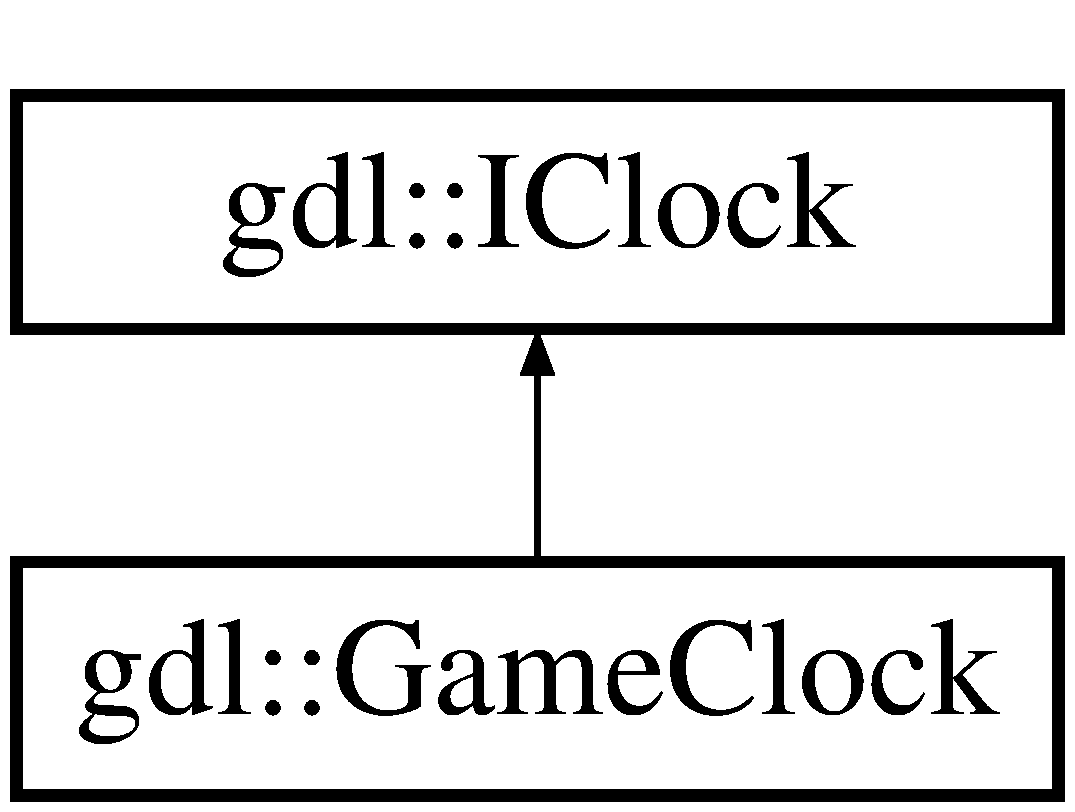
\includegraphics[height=2cm]{classgdl_1_1GameClock}
\end{center}
\end{figure}
\subsection*{Public Member Functions}
\begin{DoxyCompactItemize}
\item 
void \hyperlink{classgdl_1_1GameClock_aa7ad30c03dec94bc5b21a4fcad290644}{play} (void)
\item 
void \hyperlink{classgdl_1_1GameClock_aab85df27e686f8dbc0bcdb009a6e9158}{pause} (void)
\item 
void \hyperlink{classgdl_1_1GameClock_adb1151b518f6ee38a169b25b75542311}{update} (void)
\item 
void \hyperlink{classgdl_1_1GameClock_af568839e075e6e3c2b7aad91450d16d2}{reset} (void)
\item 
float \hyperlink{classgdl_1_1GameClock_a4c089f024d7b1448bc0d24f6a2785281}{getElapsedTime} (void) const 
\item 
float \hyperlink{classgdl_1_1GameClock_a8769e925304d57d6c6949c8bedec7956}{getTotalGameTime} (void) const 
\end{DoxyCompactItemize}
\subsection*{Friends}
\begin{DoxyCompactItemize}
\item 
\hypertarget{classgdl_1_1GameClock_aa2fab026580d6f14280c2ffb8063a314}{
class {\bfseries Game}}
\label{classgdl_1_1GameClock_aa2fab026580d6f14280c2ffb8063a314}

\end{DoxyCompactItemize}


\subsection{Detailed Description}
\hyperlink{classgdl_1_1GameClock}{GameClock} provides a main clock for the entire game. 

\subsection{Member Function Documentation}
\hypertarget{classgdl_1_1GameClock_a4c089f024d7b1448bc0d24f6a2785281}{
\index{gdl::GameClock@{gdl::GameClock}!getElapsedTime@{getElapsedTime}}
\index{getElapsedTime@{getElapsedTime}!gdl::GameClock@{gdl::GameClock}}
\subsubsection[{getElapsedTime}]{\setlength{\rightskip}{0pt plus 5cm}float gdl::GameClock::getElapsedTime (void) const\hspace{0.3cm}{\ttfamily  \mbox{[}virtual\mbox{]}}}}
\label{classgdl_1_1GameClock_a4c089f024d7b1448bc0d24f6a2785281}
Return the time since the last Update call.

\begin{DoxyReturn}{Returns}
The time in float. 
\end{DoxyReturn}


Implements \hyperlink{classgdl_1_1IClock_ad5c3e51562a10e319a3494785d077d1b}{gdl::IClock}.\hypertarget{classgdl_1_1GameClock_a8769e925304d57d6c6949c8bedec7956}{
\index{gdl::GameClock@{gdl::GameClock}!getTotalGameTime@{getTotalGameTime}}
\index{getTotalGameTime@{getTotalGameTime}!gdl::GameClock@{gdl::GameClock}}
\subsubsection[{getTotalGameTime}]{\setlength{\rightskip}{0pt plus 5cm}float gdl::GameClock::getTotalGameTime (void) const}}
\label{classgdl_1_1GameClock_a8769e925304d57d6c6949c8bedec7956}
Return the time between now and the start of the \hyperlink{classgdl_1_1Game}{Game}.

\begin{DoxyReturn}{Returns}
The time in float. 
\end{DoxyReturn}
\hypertarget{classgdl_1_1GameClock_aab85df27e686f8dbc0bcdb009a6e9158}{
\index{gdl::GameClock@{gdl::GameClock}!pause@{pause}}
\index{pause@{pause}!gdl::GameClock@{gdl::GameClock}}
\subsubsection[{pause}]{\setlength{\rightskip}{0pt plus 5cm}void gdl::GameClock::pause (void)\hspace{0.3cm}{\ttfamily  \mbox{[}virtual\mbox{]}}}}
\label{classgdl_1_1GameClock_aab85df27e686f8dbc0bcdb009a6e9158}
Stop the clock until you play it again. 

Implements \hyperlink{classgdl_1_1IClock_a7274430efa1f0e621bcce5d99d6abca7}{gdl::IClock}.\hypertarget{classgdl_1_1GameClock_aa7ad30c03dec94bc5b21a4fcad290644}{
\index{gdl::GameClock@{gdl::GameClock}!play@{play}}
\index{play@{play}!gdl::GameClock@{gdl::GameClock}}
\subsubsection[{play}]{\setlength{\rightskip}{0pt plus 5cm}void gdl::GameClock::play (void)\hspace{0.3cm}{\ttfamily  \mbox{[}virtual\mbox{]}}}}
\label{classgdl_1_1GameClock_aa7ad30c03dec94bc5b21a4fcad290644}
Start the clock. 

Implements \hyperlink{classgdl_1_1IClock_af9f70e18cd6b9b39aca1a359412adf4d}{gdl::IClock}.\hypertarget{classgdl_1_1GameClock_af568839e075e6e3c2b7aad91450d16d2}{
\index{gdl::GameClock@{gdl::GameClock}!reset@{reset}}
\index{reset@{reset}!gdl::GameClock@{gdl::GameClock}}
\subsubsection[{reset}]{\setlength{\rightskip}{0pt plus 5cm}void gdl::GameClock::reset (void)\hspace{0.3cm}{\ttfamily  \mbox{[}virtual\mbox{]}}}}
\label{classgdl_1_1GameClock_af568839e075e6e3c2b7aad91450d16d2}
Reset the clock to 0. 

Implements \hyperlink{classgdl_1_1IClock_a63cd29fcd9830e719d4cb82d5e993ec6}{gdl::IClock}.\hypertarget{classgdl_1_1GameClock_adb1151b518f6ee38a169b25b75542311}{
\index{gdl::GameClock@{gdl::GameClock}!update@{update}}
\index{update@{update}!gdl::GameClock@{gdl::GameClock}}
\subsubsection[{update}]{\setlength{\rightskip}{0pt plus 5cm}void gdl::GameClock::update (void)\hspace{0.3cm}{\ttfamily  \mbox{[}virtual\mbox{]}}}}
\label{classgdl_1_1GameClock_adb1151b518f6ee38a169b25b75542311}
Up the time of the clock. 

Implements \hyperlink{classgdl_1_1IClock_a0489f6f9055df40116e98e7ed6ad4146}{gdl::IClock}.

The documentation for this class was generated from the following files:\begin{DoxyCompactItemize}
\item 
GameClock.hpp\item 
GameClock.cpp\end{DoxyCompactItemize}

\hypertarget{classgdl_1_1IClock}{
\section{gdl::IClock Class Reference}
\label{classgdl_1_1IClock}\index{gdl::IClock@{gdl::IClock}}
}


{\ttfamily \#include $<$IClock.hpp$>$}Inheritance diagram for gdl::IClock::\begin{figure}[H]
\begin{center}
\leavevmode
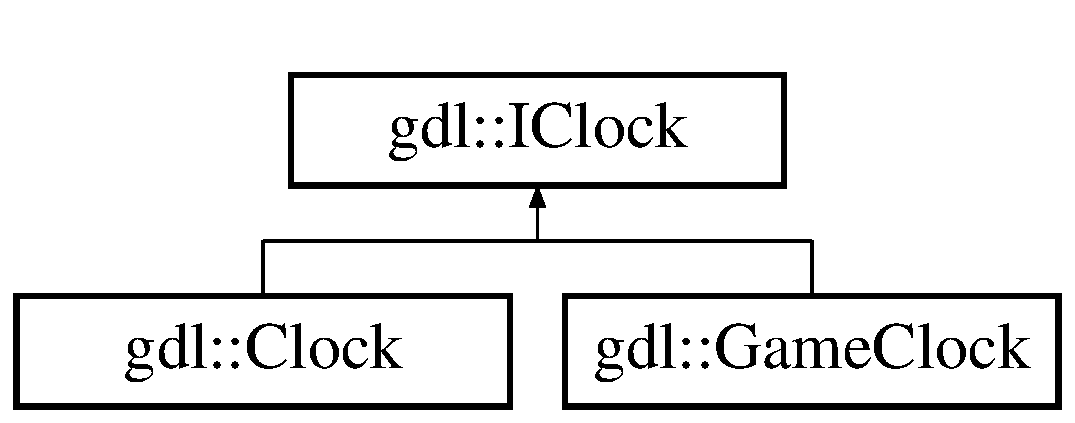
\includegraphics[height=2cm]{classgdl_1_1IClock}
\end{center}
\end{figure}
\subsection*{Public Member Functions}
\begin{DoxyCompactItemize}
\item 
virtual void \hyperlink{classgdl_1_1IClock_af9f70e18cd6b9b39aca1a359412adf4d}{play} (void)=0
\item 
virtual void \hyperlink{classgdl_1_1IClock_a7274430efa1f0e621bcce5d99d6abca7}{pause} (void)=0
\item 
virtual void \hyperlink{classgdl_1_1IClock_a0489f6f9055df40116e98e7ed6ad4146}{update} (void)=0
\item 
virtual void \hyperlink{classgdl_1_1IClock_a63cd29fcd9830e719d4cb82d5e993ec6}{reset} (void)=0
\item 
virtual float \hyperlink{classgdl_1_1IClock_ad5c3e51562a10e319a3494785d077d1b}{getElapsedTime} (void) const =0
\end{DoxyCompactItemize}


\subsection{Detailed Description}
Interface \hyperlink{classgdl_1_1IClock}{IClock} is used to force a specific time implementation. 

\subsection{Member Function Documentation}
\hypertarget{classgdl_1_1IClock_ad5c3e51562a10e319a3494785d077d1b}{
\index{gdl::IClock@{gdl::IClock}!getElapsedTime@{getElapsedTime}}
\index{getElapsedTime@{getElapsedTime}!gdl::IClock@{gdl::IClock}}
\subsubsection[{getElapsedTime}]{\setlength{\rightskip}{0pt plus 5cm}virtual float gdl::IClock::getElapsedTime (void) const\hspace{0.3cm}{\ttfamily  \mbox{[}pure virtual\mbox{]}}}}
\label{classgdl_1_1IClock_ad5c3e51562a10e319a3494785d077d1b}
Return the time between now and the last call of the update method.

\begin{DoxyReturn}{Returns}
The time in float. 
\end{DoxyReturn}


Implemented in \hyperlink{classgdl_1_1Clock_a3b81a05f6b9d4af46b6c955017c8ddfd}{gdl::Clock}, and \hyperlink{classgdl_1_1GameClock_a4c089f024d7b1448bc0d24f6a2785281}{gdl::GameClock}.\hypertarget{classgdl_1_1IClock_a7274430efa1f0e621bcce5d99d6abca7}{
\index{gdl::IClock@{gdl::IClock}!pause@{pause}}
\index{pause@{pause}!gdl::IClock@{gdl::IClock}}
\subsubsection[{pause}]{\setlength{\rightskip}{0pt plus 5cm}virtual void gdl::IClock::pause (void)\hspace{0.3cm}{\ttfamily  \mbox{[}pure virtual\mbox{]}}}}
\label{classgdl_1_1IClock_a7274430efa1f0e621bcce5d99d6abca7}
Stop the clock until you play it again. 

Implemented in \hyperlink{classgdl_1_1Clock_afcd4590e0217065f7f2c9bd13cb6c3ad}{gdl::Clock}, and \hyperlink{classgdl_1_1GameClock_aab85df27e686f8dbc0bcdb009a6e9158}{gdl::GameClock}.\hypertarget{classgdl_1_1IClock_af9f70e18cd6b9b39aca1a359412adf4d}{
\index{gdl::IClock@{gdl::IClock}!play@{play}}
\index{play@{play}!gdl::IClock@{gdl::IClock}}
\subsubsection[{play}]{\setlength{\rightskip}{0pt plus 5cm}virtual void gdl::IClock::play (void)\hspace{0.3cm}{\ttfamily  \mbox{[}pure virtual\mbox{]}}}}
\label{classgdl_1_1IClock_af9f70e18cd6b9b39aca1a359412adf4d}
Start the clock. 

Implemented in \hyperlink{classgdl_1_1Clock_af1054a354823d2556a780ddec710e368}{gdl::Clock}, and \hyperlink{classgdl_1_1GameClock_aa7ad30c03dec94bc5b21a4fcad290644}{gdl::GameClock}.\hypertarget{classgdl_1_1IClock_a63cd29fcd9830e719d4cb82d5e993ec6}{
\index{gdl::IClock@{gdl::IClock}!reset@{reset}}
\index{reset@{reset}!gdl::IClock@{gdl::IClock}}
\subsubsection[{reset}]{\setlength{\rightskip}{0pt plus 5cm}virtual void gdl::IClock::reset (void)\hspace{0.3cm}{\ttfamily  \mbox{[}pure virtual\mbox{]}}}}
\label{classgdl_1_1IClock_a63cd29fcd9830e719d4cb82d5e993ec6}
Reset the clock to 0. 

Implemented in \hyperlink{classgdl_1_1Clock_a9a44b0217d50c216d2e94d0f174e3a67}{gdl::Clock}, and \hyperlink{classgdl_1_1GameClock_af568839e075e6e3c2b7aad91450d16d2}{gdl::GameClock}.\hypertarget{classgdl_1_1IClock_a0489f6f9055df40116e98e7ed6ad4146}{
\index{gdl::IClock@{gdl::IClock}!update@{update}}
\index{update@{update}!gdl::IClock@{gdl::IClock}}
\subsubsection[{update}]{\setlength{\rightskip}{0pt plus 5cm}virtual void gdl::IClock::update (void)\hspace{0.3cm}{\ttfamily  \mbox{[}pure virtual\mbox{]}}}}
\label{classgdl_1_1IClock_a0489f6f9055df40116e98e7ed6ad4146}
Up the time of the clock. 

Implemented in \hyperlink{classgdl_1_1Clock_acc748cbe2dc79ab94c7843e2f010d049}{gdl::Clock}, and \hyperlink{classgdl_1_1GameClock_adb1151b518f6ee38a169b25b75542311}{gdl::GameClock}.

The documentation for this class was generated from the following file:\begin{DoxyCompactItemize}
\item 
IClock.hpp\end{DoxyCompactItemize}

\hypertarget{classgdl_1_1Image}{
\section{gdl::Image Class Reference}
\label{classgdl_1_1Image}\index{gdl::Image@{gdl::Image}}
}


{\ttfamily \#include $<$Image.hpp$>$}Inheritance diagram for gdl::Image::\begin{figure}[H]
\begin{center}
\leavevmode
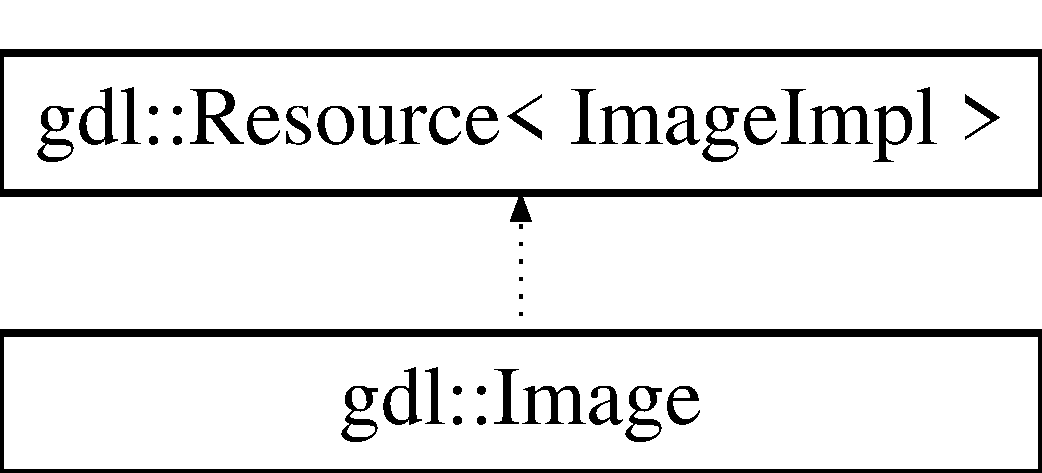
\includegraphics[height=2cm]{classgdl_1_1Image}
\end{center}
\end{figure}
\subsection*{Public Member Functions}
\begin{DoxyCompactItemize}
\item 
\hyperlink{classgdl_1_1Image_a1ccd90e38aeef3b04ee4e62ad6928b06}{Image} (void)
\item 
\hyperlink{classgdl_1_1Image_a2106e265d93d44829fe181009af0782f}{$\sim$Image} (void)
\item 
void \hyperlink{classgdl_1_1Image_a38b36eb4c9bb1ff523d56c8548e250ab}{bind} (void)
\item 
unsigned int \hyperlink{classgdl_1_1Image_afbfdaf5f3b8744d9903face66b730d93}{getWidth} (void) const 
\item 
unsigned int \hyperlink{classgdl_1_1Image_a92a2838f614afac73777e54e4a37eb4c}{getHeight} (void) const 
\item 
unsigned char const $\ast$ \hyperlink{classgdl_1_1Image_af98213f37f91724b3c5b6999864239d1}{getPixelPtr} (void) const 
\end{DoxyCompactItemize}
\subsection*{Static Public Member Functions}
\begin{DoxyCompactItemize}
\item 
static \hyperlink{classgdl_1_1Image}{Image} \hyperlink{classgdl_1_1Image_a5fbf636e446bfa53e54f6664bbe49fb7}{load} (std::string const \&filename)
\end{DoxyCompactItemize}
\subsection*{Friends}
\begin{DoxyCompactItemize}
\item 
class \hyperlink{classgdl_1_1Image_ad30335dc3a64ec73d35a335c53178345}{ImageImpl}
\end{DoxyCompactItemize}


\subsection{Detailed Description}
The \hyperlink{classgdl_1_1Image}{Image} class provides image loading and image binding. 

\subsection{Constructor \& Destructor Documentation}
\hypertarget{classgdl_1_1Image_a1ccd90e38aeef3b04ee4e62ad6928b06}{
\index{gdl::Image@{gdl::Image}!Image@{Image}}
\index{Image@{Image}!gdl::Image@{gdl::Image}}
\subsubsection[{Image}]{\setlength{\rightskip}{0pt plus 5cm}gdl::Image::Image (void)}}
\label{classgdl_1_1Image_a1ccd90e38aeef3b04ee4e62ad6928b06}
Default constructor. \hypertarget{classgdl_1_1Image_a2106e265d93d44829fe181009af0782f}{
\index{gdl::Image@{gdl::Image}!$\sim$Image@{$\sim$Image}}
\index{$\sim$Image@{$\sim$Image}!gdl::Image@{gdl::Image}}
\subsubsection[{$\sim$Image}]{\setlength{\rightskip}{0pt plus 5cm}gdl::Image::$\sim$Image (void)}}
\label{classgdl_1_1Image_a2106e265d93d44829fe181009af0782f}
Default destructor. 

\subsection{Member Function Documentation}
\hypertarget{classgdl_1_1Image_a38b36eb4c9bb1ff523d56c8548e250ab}{
\index{gdl::Image@{gdl::Image}!bind@{bind}}
\index{bind@{bind}!gdl::Image@{gdl::Image}}
\subsubsection[{bind}]{\setlength{\rightskip}{0pt plus 5cm}void gdl::Image::bind (void)}}
\label{classgdl_1_1Image_a38b36eb4c9bb1ff523d56c8548e250ab}
Bind the texture on the GPU. \hypertarget{classgdl_1_1Image_a92a2838f614afac73777e54e4a37eb4c}{
\index{gdl::Image@{gdl::Image}!getHeight@{getHeight}}
\index{getHeight@{getHeight}!gdl::Image@{gdl::Image}}
\subsubsection[{getHeight}]{\setlength{\rightskip}{0pt plus 5cm}unsigned int gdl::Image::getHeight (void) const}}
\label{classgdl_1_1Image_a92a2838f614afac73777e54e4a37eb4c}
Get the height of the image.

\begin{DoxyReturn}{Returns}
Height of the image. 
\end{DoxyReturn}
\hypertarget{classgdl_1_1Image_af98213f37f91724b3c5b6999864239d1}{
\index{gdl::Image@{gdl::Image}!getPixelPtr@{getPixelPtr}}
\index{getPixelPtr@{getPixelPtr}!gdl::Image@{gdl::Image}}
\subsubsection[{getPixelPtr}]{\setlength{\rightskip}{0pt plus 5cm}unsigned char const $\ast$ gdl::Image::getPixelPtr (void) const}}
\label{classgdl_1_1Image_af98213f37f91724b3c5b6999864239d1}
Get a pointer to the pixel array of the image.

\begin{DoxyReturn}{Returns}
Pointer to the pixel array. 
\end{DoxyReturn}
\hypertarget{classgdl_1_1Image_afbfdaf5f3b8744d9903face66b730d93}{
\index{gdl::Image@{gdl::Image}!getWidth@{getWidth}}
\index{getWidth@{getWidth}!gdl::Image@{gdl::Image}}
\subsubsection[{getWidth}]{\setlength{\rightskip}{0pt plus 5cm}unsigned int gdl::Image::getWidth (void) const}}
\label{classgdl_1_1Image_afbfdaf5f3b8744d9903face66b730d93}
Get the width of the image.

\begin{DoxyReturn}{Returns}
Width of the image. 
\end{DoxyReturn}
\hypertarget{classgdl_1_1Image_a5fbf636e446bfa53e54f6664bbe49fb7}{
\index{gdl::Image@{gdl::Image}!load@{load}}
\index{load@{load}!gdl::Image@{gdl::Image}}
\subsubsection[{load}]{\setlength{\rightskip}{0pt plus 5cm}{\bf Image} gdl::Image::load (std::string const \& {\em filename})\hspace{0.3cm}{\ttfamily  \mbox{[}static\mbox{]}}}}
\label{classgdl_1_1Image_a5fbf636e446bfa53e54f6664bbe49fb7}
Load an image from a file.


\begin{DoxyParams}{Parameters}
\item[\mbox{$\leftarrow$} {\em filename}]Filename of the image with extension. \end{DoxyParams}
\begin{DoxyReturn}{Returns}
An instance of the resource. 
\end{DoxyReturn}


\subsection{Friends And Related Function Documentation}
\hypertarget{classgdl_1_1Image_ad30335dc3a64ec73d35a335c53178345}{
\index{gdl::Image@{gdl::Image}!ImageImpl@{ImageImpl}}
\index{ImageImpl@{ImageImpl}!gdl::Image@{gdl::Image}}
\subsubsection[{ImageImpl}]{\setlength{\rightskip}{0pt plus 5cm}friend class ImageImpl\hspace{0.3cm}{\ttfamily  \mbox{[}friend\mbox{]}}}}
\label{classgdl_1_1Image_ad30335dc3a64ec73d35a335c53178345}
\hyperlink{classgdl_1_1Image}{Image} implementation. 

The documentation for this class was generated from the following files:\begin{DoxyCompactItemize}
\item 
Image.hpp\item 
Image.cpp\end{DoxyCompactItemize}

\hypertarget{classgdl_1_1Input}{
\section{gdl::Input Class Reference}
\label{classgdl_1_1Input}\index{gdl::Input@{gdl::Input}}
}


{\ttfamily \#include $<$Input.hpp$>$}\subsection*{Public Member Functions}
\begin{DoxyCompactItemize}
\item 
\hyperlink{classgdl_1_1Input_aaaec080ed208c7a0e93160e11710a6db}{Input} (\hyperlink{classgdl_1_1Window}{gdl::Window} \&window)
\item 
\hyperlink{classgdl_1_1Input_aa9c7fd004ef583434b65ddf7ebbad9bc}{$\sim$Input} ()
\item 
bool \hyperlink{classgdl_1_1Input_ae0bfa17187848fd6a1576eb1e8204230}{isKeyDown} (gdl::Keys::Key key)
\item 
bool \hyperlink{classgdl_1_1Input_a893c44e94392d6d2d3c01f5ff4263f96}{isMouseButtonDown} (gdl::Mouse::Button button)
\item 
int \hyperlink{classgdl_1_1Input_a1a9f9de83134c8ea6e62ece2163868ca}{getMousePositionX} (void) const 
\item 
int \hyperlink{classgdl_1_1Input_a8732662c038df92f1cb422973b675288}{getMousePositionY} (void) const 
\end{DoxyCompactItemize}


\subsection{Detailed Description}
The \hyperlink{classgdl_1_1Input}{Input} class catches each input event for a window. 

\subsection{Constructor \& Destructor Documentation}
\hypertarget{classgdl_1_1Input_aaaec080ed208c7a0e93160e11710a6db}{
\index{gdl::Input@{gdl::Input}!Input@{Input}}
\index{Input@{Input}!gdl::Input@{gdl::Input}}
\subsubsection[{Input}]{\setlength{\rightskip}{0pt plus 5cm}gdl::Input::Input ({\bf gdl::Window} \& {\em window})}}
\label{classgdl_1_1Input_aaaec080ed208c7a0e93160e11710a6db}
Constructor.


\begin{DoxyParams}{Parameters}
\item[\mbox{$\leftarrow$} {\em window}]\hyperlink{classgdl_1_1Window}{Window} to link with. \end{DoxyParams}
\hypertarget{classgdl_1_1Input_aa9c7fd004ef583434b65ddf7ebbad9bc}{
\index{gdl::Input@{gdl::Input}!$\sim$Input@{$\sim$Input}}
\index{$\sim$Input@{$\sim$Input}!gdl::Input@{gdl::Input}}
\subsubsection[{$\sim$Input}]{\setlength{\rightskip}{0pt plus 5cm}gdl::Input::$\sim$Input ()}}
\label{classgdl_1_1Input_aa9c7fd004ef583434b65ddf7ebbad9bc}
Default destructor. 

\subsection{Member Function Documentation}
\hypertarget{classgdl_1_1Input_a1a9f9de83134c8ea6e62ece2163868ca}{
\index{gdl::Input@{gdl::Input}!getMousePositionX@{getMousePositionX}}
\index{getMousePositionX@{getMousePositionX}!gdl::Input@{gdl::Input}}
\subsubsection[{getMousePositionX}]{\setlength{\rightskip}{0pt plus 5cm}int gdl::Input::getMousePositionX (void) const}}
\label{classgdl_1_1Input_a1a9f9de83134c8ea6e62ece2163868ca}
Get the cursor position.

\begin{DoxyReturn}{Returns}
The cursor position on x-\/axis. 
\end{DoxyReturn}
\hypertarget{classgdl_1_1Input_a8732662c038df92f1cb422973b675288}{
\index{gdl::Input@{gdl::Input}!getMousePositionY@{getMousePositionY}}
\index{getMousePositionY@{getMousePositionY}!gdl::Input@{gdl::Input}}
\subsubsection[{getMousePositionY}]{\setlength{\rightskip}{0pt plus 5cm}int gdl::Input::getMousePositionY (void) const}}
\label{classgdl_1_1Input_a8732662c038df92f1cb422973b675288}
Get the cursor position.

\begin{DoxyReturn}{Returns}
The cursor position on y-\/axis. 
\end{DoxyReturn}
\hypertarget{classgdl_1_1Input_ae0bfa17187848fd6a1576eb1e8204230}{
\index{gdl::Input@{gdl::Input}!isKeyDown@{isKeyDown}}
\index{isKeyDown@{isKeyDown}!gdl::Input@{gdl::Input}}
\subsubsection[{isKeyDown}]{\setlength{\rightskip}{0pt plus 5cm}bool gdl::Input::isKeyDown (gdl::Keys::Key {\em key})}}
\label{classgdl_1_1Input_ae0bfa17187848fd6a1576eb1e8204230}
Check if a key is down.


\begin{DoxyParams}{Parameters}
\item[\mbox{$\leftarrow$} {\em key}]Key to check. \end{DoxyParams}
\begin{DoxyReturn}{Returns}
If the key is down, true is returned. Otherwise, returned false. 
\end{DoxyReturn}
\hypertarget{classgdl_1_1Input_a893c44e94392d6d2d3c01f5ff4263f96}{
\index{gdl::Input@{gdl::Input}!isMouseButtonDown@{isMouseButtonDown}}
\index{isMouseButtonDown@{isMouseButtonDown}!gdl::Input@{gdl::Input}}
\subsubsection[{isMouseButtonDown}]{\setlength{\rightskip}{0pt plus 5cm}bool gdl::Input::isMouseButtonDown (gdl::Mouse::Button {\em button})}}
\label{classgdl_1_1Input_a893c44e94392d6d2d3c01f5ff4263f96}
Check if a mouse button is down.


\begin{DoxyParams}{Parameters}
\item[\mbox{$\leftarrow$} {\em button}]Button to check. \end{DoxyParams}
\begin{DoxyReturn}{Returns}
If the button is down, true is returned. Otherwise, returned false. 
\end{DoxyReturn}


The documentation for this class was generated from the following files:\begin{DoxyCompactItemize}
\item 
Input.hpp\item 
Input.cpp\end{DoxyCompactItemize}

\hypertarget{classgdl_1_1Model}{
\section{gdl::Model Class Reference}
\label{classgdl_1_1Model}\index{gdl::Model@{gdl::Model}}
}


{\ttfamily \#include $<$Model.hpp$>$}Inheritance diagram for gdl::Model::\begin{figure}[H]
\begin{center}
\leavevmode
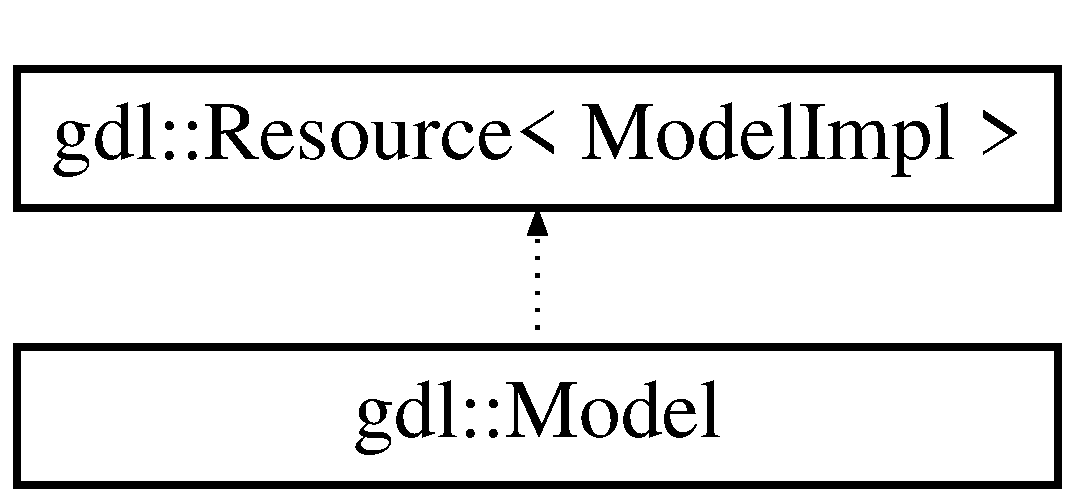
\includegraphics[height=2cm]{classgdl_1_1Model}
\end{center}
\end{figure}
\subsection*{Public Member Functions}
\begin{DoxyCompactItemize}
\item 
\hyperlink{classgdl_1_1Model_a48d0cb59ef4926b95b1a4504d6b6fbe0}{Model} (void)
\item 
\hyperlink{classgdl_1_1Model_a76ba0ddf7db67016d0a72f0c22febca4}{$\sim$Model} (void)
\item 
void \hyperlink{classgdl_1_1Model_a9e5a520c27759a0913010e88262f87d0}{update} (\hyperlink{classgdl_1_1IClock}{IClock} const \&gameTime)
\item 
void \hyperlink{classgdl_1_1Model_af8cbb946c57ab177273521bb3c127fb4}{draw} (void)
\item 
void \hyperlink{classgdl_1_1Model_a4835d0ce38b458dc0b378f4a025c5a09}{draw\_\-pose} (int pose\_\-id)
\item 
void \hyperlink{classgdl_1_1Model_ae767b95441e66f3c5e8f06efd6f785fe}{infos} (void)
\item 
bool \hyperlink{classgdl_1_1Model_abd7249531d6433c6a8c0970f931b16e6}{play} (std::string const \&\_\-name, char state=Anim::RUN)
\item 
bool \hyperlink{classgdl_1_1Model_a5046ca0821ca4c5a6a6ec33c51b41903}{animation\_\-hasStarted} (std::string const \&name) const 
\item 
bool \hyperlink{classgdl_1_1Model_a3fcf22fc2e37057fe047c3841d30c88b}{anim\_\-is\_\-ended} (std::string const \&name) const 
\item 
void \hyperlink{classgdl_1_1Model_a565112440d65142e71911e60cdb223bb}{stop\_\-animation} (std::string const \&name)
\item 
double \hyperlink{classgdl_1_1Model_a5ccf274812bacb19062d4051fbe44b57}{get\_\-anim\_\-speed} (std::string const \&name) const 
\item 
double \hyperlink{classgdl_1_1Model_a97d6d0d3f9e6df95e20caf26e769bea4}{get\_\-anim\_\-blendfactor} (std::string const \&name) const 
\item 
char \hyperlink{classgdl_1_1Model_a5cb4cfea0c7f0819d0749baddd682f98}{get\_\-anim\_\-state} (std::string const \&name) const 
\item 
void \hyperlink{classgdl_1_1Model_a0cbcdc21c1962e7230fcba6b063b119a}{set\_\-anim\_\-bendfactor} (std::string const \&name, double blendFactor)
\item 
void \hyperlink{classgdl_1_1Model_abebb3405288cef12250671957cda4925}{set\_\-anim\_\-speed} (std::string const \&name, double speed)
\item 
\hyperlink{structgdl_1_1Color}{Color} const \& \hyperlink{classgdl_1_1Model_a8bbdffaebc6ef023b84d609d9f00a43e}{get\_\-default\_\-model\_\-color} (void) const 
\item 
void \hyperlink{classgdl_1_1Model_a5fe9cd2cbfe7a993505528832cdc0604}{set\_\-default\_\-model\_\-color} (\hyperlink{structgdl_1_1Color}{Color} const \&color)
\item 
void \hyperlink{classgdl_1_1Model_a7239d032a682d61fcf69194e34461102}{set\_\-anim\_\-state} (std::string const \&name, char state)
\item 
void \hyperlink{classgdl_1_1Model_a2bf37d490e0dd0906d4ee7d74aca5df3}{add\_\-anim\_\-state} (std::string const \&name, Anim::AnimStates state)
\item 
void \hyperlink{classgdl_1_1Model_af32a30b8fc163e1dc9d1a78eff49f2ea}{remove\_\-anim\_\-state} (std::string const \&name, Anim::AnimStates state)
\item 
std::vector$<$ std::string $>$ const \& \hyperlink{classgdl_1_1Model_accd5847c295adfc7cebcd2283ee2bfdf}{get\_\-stackanimation\_\-names} (void) const 
\item 
std::vector$<$ std::string $>$ const \& \hyperlink{classgdl_1_1Model_a7f09fd45a42fd3314e320c0b969ab2bc}{get\_\-animation\_\-names} (void) const 
\end{DoxyCompactItemize}
\subsection*{Static Public Member Functions}
\begin{DoxyCompactItemize}
\item 
static \hyperlink{classgdl_1_1Model}{Model} \hyperlink{classgdl_1_1Model_a6f9c70f0e5b0b0c640d739a4fd1249cd}{load} (std::string const \&filename)
\item 
static bool \hyperlink{classgdl_1_1Model_ad477ab8d1ffe487499886170a1b0d949}{cut\_\-animation} (\hyperlink{classgdl_1_1Model}{Model} \&\_\-model, std::string const \&stackAnim, int id\_\-start, int id\_\-end, std::string const \&\_\-newName)
\item 
static void \hyperlink{classgdl_1_1Model_ae1ede142757404fb1869c62c682bc48b}{Begin} (void)
\item 
static void \hyperlink{classgdl_1_1Model_a65b3733d5447e12316befa7a28eeadd7}{End} (void)
\end{DoxyCompactItemize}
\subsection*{Friends}
\begin{DoxyCompactItemize}
\item 
class \hyperlink{classgdl_1_1Model_afb81d2077780e342b8fd3654cabc4c19}{ModelImpl}
\item 
class \hyperlink{classgdl_1_1Model_a7afc1a807b9064f725fdcdce33639acb}{ResourceManagerImpl}
\end{DoxyCompactItemize}


\subsection{Detailed Description}
The ModelImpl class provide the gestion of your model. 

\subsection{Constructor \& Destructor Documentation}
\hypertarget{classgdl_1_1Model_a48d0cb59ef4926b95b1a4504d6b6fbe0}{
\index{gdl::Model@{gdl::Model}!Model@{Model}}
\index{Model@{Model}!gdl::Model@{gdl::Model}}
\subsubsection[{Model}]{\setlength{\rightskip}{0pt plus 5cm}gdl::Model::Model (void)}}
\label{classgdl_1_1Model_a48d0cb59ef4926b95b1a4504d6b6fbe0}
Default constructror. \hypertarget{classgdl_1_1Model_a76ba0ddf7db67016d0a72f0c22febca4}{
\index{gdl::Model@{gdl::Model}!$\sim$Model@{$\sim$Model}}
\index{$\sim$Model@{$\sim$Model}!gdl::Model@{gdl::Model}}
\subsubsection[{$\sim$Model}]{\setlength{\rightskip}{0pt plus 5cm}gdl::Model::$\sim$Model (void)}}
\label{classgdl_1_1Model_a76ba0ddf7db67016d0a72f0c22febca4}
Default destructror. 

\subsection{Member Function Documentation}
\hypertarget{classgdl_1_1Model_a2bf37d490e0dd0906d4ee7d74aca5df3}{
\index{gdl::Model@{gdl::Model}!add\_\-anim\_\-state@{add\_\-anim\_\-state}}
\index{add\_\-anim\_\-state@{add\_\-anim\_\-state}!gdl::Model@{gdl::Model}}
\subsubsection[{add\_\-anim\_\-state}]{\setlength{\rightskip}{0pt plus 5cm}void gdl::Model::add\_\-anim\_\-state (std::string const \& {\em name}, \/  Anim::AnimStates {\em state})}}
\label{classgdl_1_1Model_a2bf37d490e0dd0906d4ee7d74aca5df3}
Add an animation state.


\begin{DoxyParams}{Parameters}
\item[\mbox{$\leftarrow$} {\em name}]Animation name. \item[\mbox{$\leftarrow$} {\em state}](in Anim namespace). \end{DoxyParams}
\hypertarget{classgdl_1_1Model_a3fcf22fc2e37057fe047c3841d30c88b}{
\index{gdl::Model@{gdl::Model}!anim\_\-is\_\-ended@{anim\_\-is\_\-ended}}
\index{anim\_\-is\_\-ended@{anim\_\-is\_\-ended}!gdl::Model@{gdl::Model}}
\subsubsection[{anim\_\-is\_\-ended}]{\setlength{\rightskip}{0pt plus 5cm}bool gdl::Model::anim\_\-is\_\-ended (std::string const \& {\em name}) const}}
\label{classgdl_1_1Model_a3fcf22fc2e37057fe047c3841d30c88b}
Check if the animation is ended.


\begin{DoxyParams}{Parameters}
\item[\mbox{$\leftarrow$} {\em name}]Animation name. \end{DoxyParams}
\begin{DoxyReturn}{Returns}
If the animation has ended, true is returned. Otherwise, false is returned. 
\end{DoxyReturn}
\hypertarget{classgdl_1_1Model_a5046ca0821ca4c5a6a6ec33c51b41903}{
\index{gdl::Model@{gdl::Model}!animation\_\-hasStarted@{animation\_\-hasStarted}}
\index{animation\_\-hasStarted@{animation\_\-hasStarted}!gdl::Model@{gdl::Model}}
\subsubsection[{animation\_\-hasStarted}]{\setlength{\rightskip}{0pt plus 5cm}bool gdl::Model::animation\_\-hasStarted (std::string const \& {\em name}) const}}
\label{classgdl_1_1Model_a5046ca0821ca4c5a6a6ec33c51b41903}
Check if the animation has started.


\begin{DoxyParams}{Parameters}
\item[{\em name}]Animation name. \end{DoxyParams}
\begin{DoxyReturn}{Returns}
If successful, true is returned. Otherwise, false is returned. 
\end{DoxyReturn}
\hypertarget{classgdl_1_1Model_ae1ede142757404fb1869c62c682bc48b}{
\index{gdl::Model@{gdl::Model}!Begin@{Begin}}
\index{Begin@{Begin}!gdl::Model@{gdl::Model}}
\subsubsection[{Begin}]{\setlength{\rightskip}{0pt plus 5cm}void gdl::Model::Begin (void)\hspace{0.3cm}{\ttfamily  \mbox{[}static\mbox{]}}}}
\label{classgdl_1_1Model_ae1ede142757404fb1869c62c682bc48b}
Open the scope to draw models. \hypertarget{classgdl_1_1Model_ad477ab8d1ffe487499886170a1b0d949}{
\index{gdl::Model@{gdl::Model}!cut\_\-animation@{cut\_\-animation}}
\index{cut\_\-animation@{cut\_\-animation}!gdl::Model@{gdl::Model}}
\subsubsection[{cut\_\-animation}]{\setlength{\rightskip}{0pt plus 5cm}bool gdl::Model::cut\_\-animation ({\bf Model} \& {\em \_\-model}, \/  std::string const \& {\em stackAnim}, \/  int {\em id\_\-start}, \/  int {\em id\_\-end}, \/  std::string const \& {\em \_\-newName})\hspace{0.3cm}{\ttfamily  \mbox{[}static\mbox{]}}}}
\label{classgdl_1_1Model_ad477ab8d1ffe487499886170a1b0d949}
Cut the animation.


\begin{DoxyParams}{Parameters}
\item[\mbox{$\leftarrow$} {\em \_\-model}]The model. \item[\mbox{$\leftarrow$} {\em stackAnim}]The animations stack. \item[\mbox{$\leftarrow$} {\em id\_\-start}]First id. \item[\mbox{$\leftarrow$} {\em id\_\-end}]Last id. \item[\mbox{$\leftarrow$} {\em \_\-newName}]Name of the new animation. \end{DoxyParams}
\begin{DoxyReturn}{Returns}
If successfull, true is returned. Otherwise, false is returned. 
\end{DoxyReturn}
\hypertarget{classgdl_1_1Model_af8cbb946c57ab177273521bb3c127fb4}{
\index{gdl::Model@{gdl::Model}!draw@{draw}}
\index{draw@{draw}!gdl::Model@{gdl::Model}}
\subsubsection[{draw}]{\setlength{\rightskip}{0pt plus 5cm}void gdl::Model::draw (void)}}
\label{classgdl_1_1Model_af8cbb946c57ab177273521bb3c127fb4}
Draw the model in the \hyperlink{classgdl_1_1Window}{Window}. \hypertarget{classgdl_1_1Model_a4835d0ce38b458dc0b378f4a025c5a09}{
\index{gdl::Model@{gdl::Model}!draw\_\-pose@{draw\_\-pose}}
\index{draw\_\-pose@{draw\_\-pose}!gdl::Model@{gdl::Model}}
\subsubsection[{draw\_\-pose}]{\setlength{\rightskip}{0pt plus 5cm}void gdl::Model::draw\_\-pose (int {\em pose\_\-id})}}
\label{classgdl_1_1Model_a4835d0ce38b458dc0b378f4a025c5a09}
Draw the model in a specific pose.


\begin{DoxyParams}{Parameters}
\item[\mbox{$\leftarrow$} {\em pose\_\-id}]ID of the specific pose. \end{DoxyParams}
\hypertarget{classgdl_1_1Model_a65b3733d5447e12316befa7a28eeadd7}{
\index{gdl::Model@{gdl::Model}!End@{End}}
\index{End@{End}!gdl::Model@{gdl::Model}}
\subsubsection[{End}]{\setlength{\rightskip}{0pt plus 5cm}void gdl::Model::End (void)\hspace{0.3cm}{\ttfamily  \mbox{[}static\mbox{]}}}}
\label{classgdl_1_1Model_a65b3733d5447e12316befa7a28eeadd7}
Close the scope to draw models. \hypertarget{classgdl_1_1Model_a97d6d0d3f9e6df95e20caf26e769bea4}{
\index{gdl::Model@{gdl::Model}!get\_\-anim\_\-blendfactor@{get\_\-anim\_\-blendfactor}}
\index{get\_\-anim\_\-blendfactor@{get\_\-anim\_\-blendfactor}!gdl::Model@{gdl::Model}}
\subsubsection[{get\_\-anim\_\-blendfactor}]{\setlength{\rightskip}{0pt plus 5cm}double gdl::Model::get\_\-anim\_\-blendfactor (std::string const \& {\em name}) const}}
\label{classgdl_1_1Model_a97d6d0d3f9e6df95e20caf26e769bea4}
Get the blend factor.


\begin{DoxyParams}{Parameters}
\item[\mbox{$\leftarrow$} {\em name}]Animation name. \end{DoxyParams}
\begin{DoxyReturn}{Returns}
If the animation doesn't exist, -\/1 is returned. 
\end{DoxyReturn}
\hypertarget{classgdl_1_1Model_a5ccf274812bacb19062d4051fbe44b57}{
\index{gdl::Model@{gdl::Model}!get\_\-anim\_\-speed@{get\_\-anim\_\-speed}}
\index{get\_\-anim\_\-speed@{get\_\-anim\_\-speed}!gdl::Model@{gdl::Model}}
\subsubsection[{get\_\-anim\_\-speed}]{\setlength{\rightskip}{0pt plus 5cm}double gdl::Model::get\_\-anim\_\-speed (std::string const \& {\em name}) const}}
\label{classgdl_1_1Model_a5ccf274812bacb19062d4051fbe44b57}
Get the animation speed.


\begin{DoxyParams}{Parameters}
\item[\mbox{$\leftarrow$} {\em name}]Animation name. \end{DoxyParams}
\begin{DoxyReturn}{Returns}
If the animation doesn't exist, -\/1 is returned. 
\end{DoxyReturn}
\hypertarget{classgdl_1_1Model_a5cb4cfea0c7f0819d0749baddd682f98}{
\index{gdl::Model@{gdl::Model}!get\_\-anim\_\-state@{get\_\-anim\_\-state}}
\index{get\_\-anim\_\-state@{get\_\-anim\_\-state}!gdl::Model@{gdl::Model}}
\subsubsection[{get\_\-anim\_\-state}]{\setlength{\rightskip}{0pt plus 5cm}char gdl::Model::get\_\-anim\_\-state (std::string const \& {\em name}) const}}
\label{classgdl_1_1Model_a5cb4cfea0c7f0819d0749baddd682f98}
Get the anim state.


\begin{DoxyParams}{Parameters}
\item[\mbox{$\leftarrow$} {\em name}]Animation name. \end{DoxyParams}
\begin{DoxyReturn}{Returns}
If the animation doesn't exist, -\/1 is returned. 
\end{DoxyReturn}
\hypertarget{classgdl_1_1Model_a7f09fd45a42fd3314e320c0b969ab2bc}{
\index{gdl::Model@{gdl::Model}!get\_\-animation\_\-names@{get\_\-animation\_\-names}}
\index{get\_\-animation\_\-names@{get\_\-animation\_\-names}!gdl::Model@{gdl::Model}}
\subsubsection[{get\_\-animation\_\-names}]{\setlength{\rightskip}{0pt plus 5cm}std::vector$<$ std::string $>$ const \& gdl::Model::get\_\-animation\_\-names (void) const}}
\label{classgdl_1_1Model_a7f09fd45a42fd3314e320c0b969ab2bc}
Get the animation's name.

\begin{DoxyReturn}{Returns}
Vector of strings. 
\end{DoxyReturn}
\hypertarget{classgdl_1_1Model_a8bbdffaebc6ef023b84d609d9f00a43e}{
\index{gdl::Model@{gdl::Model}!get\_\-default\_\-model\_\-color@{get\_\-default\_\-model\_\-color}}
\index{get\_\-default\_\-model\_\-color@{get\_\-default\_\-model\_\-color}!gdl::Model@{gdl::Model}}
\subsubsection[{get\_\-default\_\-model\_\-color}]{\setlength{\rightskip}{0pt plus 5cm}const {\bf Color} \& gdl::Model::get\_\-default\_\-model\_\-color (void) const}}
\label{classgdl_1_1Model_a8bbdffaebc6ef023b84d609d9f00a43e}
Get the default model color.

\begin{DoxyReturn}{Returns}
The default color. 
\end{DoxyReturn}
\hypertarget{classgdl_1_1Model_accd5847c295adfc7cebcd2283ee2bfdf}{
\index{gdl::Model@{gdl::Model}!get\_\-stackanimation\_\-names@{get\_\-stackanimation\_\-names}}
\index{get\_\-stackanimation\_\-names@{get\_\-stackanimation\_\-names}!gdl::Model@{gdl::Model}}
\subsubsection[{get\_\-stackanimation\_\-names}]{\setlength{\rightskip}{0pt plus 5cm}std::vector$<$ std::string $>$ const \& gdl::Model::get\_\-stackanimation\_\-names (void) const}}
\label{classgdl_1_1Model_accd5847c295adfc7cebcd2283ee2bfdf}
Get the stack of the animation's name.

\begin{DoxyReturn}{Returns}
Vector of strings. 
\end{DoxyReturn}
\hypertarget{classgdl_1_1Model_ae767b95441e66f3c5e8f06efd6f785fe}{
\index{gdl::Model@{gdl::Model}!infos@{infos}}
\index{infos@{infos}!gdl::Model@{gdl::Model}}
\subsubsection[{infos}]{\setlength{\rightskip}{0pt plus 5cm}void gdl::Model::infos (void)}}
\label{classgdl_1_1Model_ae767b95441e66f3c5e8f06efd6f785fe}
Do nothing. Have to display informations about the \hyperlink{classgdl_1_1Model}{Model} like stack anime number, vertices number... \hypertarget{classgdl_1_1Model_a6f9c70f0e5b0b0c640d739a4fd1249cd}{
\index{gdl::Model@{gdl::Model}!load@{load}}
\index{load@{load}!gdl::Model@{gdl::Model}}
\subsubsection[{load}]{\setlength{\rightskip}{0pt plus 5cm}{\bf Model} gdl::Model::load (std::string const \& {\em filename})\hspace{0.3cm}{\ttfamily  \mbox{[}static\mbox{]}}}}
\label{classgdl_1_1Model_a6f9c70f0e5b0b0c640d739a4fd1249cd}
Load the model.


\begin{DoxyParams}{Parameters}
\item[\mbox{$\leftarrow$} {\em filename}]Filename with the extension. \end{DoxyParams}
\begin{DoxyReturn}{Returns}
the \hyperlink{classgdl_1_1Model}{Model}. 
\end{DoxyReturn}
\hypertarget{classgdl_1_1Model_abd7249531d6433c6a8c0970f931b16e6}{
\index{gdl::Model@{gdl::Model}!play@{play}}
\index{play@{play}!gdl::Model@{gdl::Model}}
\subsubsection[{play}]{\setlength{\rightskip}{0pt plus 5cm}bool gdl::Model::play (std::string const \& {\em \_\-name}, \/  char {\em state} = {\ttfamily Anim::RUN})}}
\label{classgdl_1_1Model_abd7249531d6433c6a8c0970f931b16e6}
Play the animation.


\begin{DoxyParams}{Parameters}
\item[\mbox{$\leftarrow$} {\em \_\-name}]Animation name. \item[\mbox{$\leftarrow$} {\em state}](AnimState enum). \end{DoxyParams}
\begin{DoxyReturn}{Returns}
If successful, true is returned. Otherwise, false is returned. 
\end{DoxyReturn}
\hypertarget{classgdl_1_1Model_af32a30b8fc163e1dc9d1a78eff49f2ea}{
\index{gdl::Model@{gdl::Model}!remove\_\-anim\_\-state@{remove\_\-anim\_\-state}}
\index{remove\_\-anim\_\-state@{remove\_\-anim\_\-state}!gdl::Model@{gdl::Model}}
\subsubsection[{remove\_\-anim\_\-state}]{\setlength{\rightskip}{0pt plus 5cm}void gdl::Model::remove\_\-anim\_\-state (std::string const \& {\em name}, \/  Anim::AnimStates {\em state})}}
\label{classgdl_1_1Model_af32a30b8fc163e1dc9d1a78eff49f2ea}
Remove an animation state.


\begin{DoxyParams}{Parameters}
\item[\mbox{$\leftarrow$} {\em name}]Animation name. \item[\mbox{$\leftarrow$} {\em state}](in Anim namespace). \end{DoxyParams}
\hypertarget{classgdl_1_1Model_a0cbcdc21c1962e7230fcba6b063b119a}{
\index{gdl::Model@{gdl::Model}!set\_\-anim\_\-bendfactor@{set\_\-anim\_\-bendfactor}}
\index{set\_\-anim\_\-bendfactor@{set\_\-anim\_\-bendfactor}!gdl::Model@{gdl::Model}}
\subsubsection[{set\_\-anim\_\-bendfactor}]{\setlength{\rightskip}{0pt plus 5cm}void gdl::Model::set\_\-anim\_\-bendfactor (std::string const \& {\em name}, \/  double {\em blendFactor})}}
\label{classgdl_1_1Model_a0cbcdc21c1962e7230fcba6b063b119a}
Set the blend factor.


\begin{DoxyParams}{Parameters}
\item[\mbox{$\leftarrow$} {\em name}]Animation name. \item[\mbox{$\leftarrow$} {\em blendFactor}]Blend factor. \end{DoxyParams}
\hypertarget{classgdl_1_1Model_abebb3405288cef12250671957cda4925}{
\index{gdl::Model@{gdl::Model}!set\_\-anim\_\-speed@{set\_\-anim\_\-speed}}
\index{set\_\-anim\_\-speed@{set\_\-anim\_\-speed}!gdl::Model@{gdl::Model}}
\subsubsection[{set\_\-anim\_\-speed}]{\setlength{\rightskip}{0pt plus 5cm}void gdl::Model::set\_\-anim\_\-speed (std::string const \& {\em name}, \/  double {\em speed})}}
\label{classgdl_1_1Model_abebb3405288cef12250671957cda4925}
Set the animation speed.


\begin{DoxyParams}{Parameters}
\item[\mbox{$\leftarrow$} {\em name}]Animation name. \item[\mbox{$\leftarrow$} {\em speed}]Speed of the animation. \end{DoxyParams}
\hypertarget{classgdl_1_1Model_a7239d032a682d61fcf69194e34461102}{
\index{gdl::Model@{gdl::Model}!set\_\-anim\_\-state@{set\_\-anim\_\-state}}
\index{set\_\-anim\_\-state@{set\_\-anim\_\-state}!gdl::Model@{gdl::Model}}
\subsubsection[{set\_\-anim\_\-state}]{\setlength{\rightskip}{0pt plus 5cm}void gdl::Model::set\_\-anim\_\-state (std::string const \& {\em name}, \/  char {\em state})}}
\label{classgdl_1_1Model_a7239d032a682d61fcf69194e34461102}
Set the anim state.


\begin{DoxyParams}{Parameters}
\item[\mbox{$\leftarrow$} {\em name}]Animation name. \item[\mbox{$\leftarrow$} {\em state}](with AnimState enum). \end{DoxyParams}
\hypertarget{classgdl_1_1Model_a5fe9cd2cbfe7a993505528832cdc0604}{
\index{gdl::Model@{gdl::Model}!set\_\-default\_\-model\_\-color@{set\_\-default\_\-model\_\-color}}
\index{set\_\-default\_\-model\_\-color@{set\_\-default\_\-model\_\-color}!gdl::Model@{gdl::Model}}
\subsubsection[{set\_\-default\_\-model\_\-color}]{\setlength{\rightskip}{0pt plus 5cm}void gdl::Model::set\_\-default\_\-model\_\-color ({\bf Color} const \& {\em color})}}
\label{classgdl_1_1Model_a5fe9cd2cbfe7a993505528832cdc0604}
Set the default model color.


\begin{DoxyParams}{Parameters}
\item[\mbox{$\leftarrow$} {\em color}]The default color. \end{DoxyParams}
\hypertarget{classgdl_1_1Model_a565112440d65142e71911e60cdb223bb}{
\index{gdl::Model@{gdl::Model}!stop\_\-animation@{stop\_\-animation}}
\index{stop\_\-animation@{stop\_\-animation}!gdl::Model@{gdl::Model}}
\subsubsection[{stop\_\-animation}]{\setlength{\rightskip}{0pt plus 5cm}void gdl::Model::stop\_\-animation (std::string const \& {\em name})}}
\label{classgdl_1_1Model_a565112440d65142e71911e60cdb223bb}
Stop the animation.


\begin{DoxyParams}{Parameters}
\item[\mbox{$\leftarrow$} {\em name}]Animation name. \end{DoxyParams}
\hypertarget{classgdl_1_1Model_a9e5a520c27759a0913010e88262f87d0}{
\index{gdl::Model@{gdl::Model}!update@{update}}
\index{update@{update}!gdl::Model@{gdl::Model}}
\subsubsection[{update}]{\setlength{\rightskip}{0pt plus 5cm}void gdl::Model::update ({\bf IClock} const \& {\em gameTime})}}
\label{classgdl_1_1Model_a9e5a520c27759a0913010e88262f87d0}
Update the animation of the model.


\begin{DoxyParams}{Parameters}
\item[\mbox{$\leftarrow$} {\em gameTime}]Game's clock. \end{DoxyParams}


\subsection{Friends And Related Function Documentation}
\hypertarget{classgdl_1_1Model_afb81d2077780e342b8fd3654cabc4c19}{
\index{gdl::Model@{gdl::Model}!ModelImpl@{ModelImpl}}
\index{ModelImpl@{ModelImpl}!gdl::Model@{gdl::Model}}
\subsubsection[{ModelImpl}]{\setlength{\rightskip}{0pt plus 5cm}friend class ModelImpl\hspace{0.3cm}{\ttfamily  \mbox{[}friend\mbox{]}}}}
\label{classgdl_1_1Model_afb81d2077780e342b8fd3654cabc4c19}
To reach private members of ModelImpl. \hypertarget{classgdl_1_1Model_a7afc1a807b9064f725fdcdce33639acb}{
\index{gdl::Model@{gdl::Model}!ResourceManagerImpl@{ResourceManagerImpl}}
\index{ResourceManagerImpl@{ResourceManagerImpl}!gdl::Model@{gdl::Model}}
\subsubsection[{ResourceManagerImpl}]{\setlength{\rightskip}{0pt plus 5cm}friend class ResourceManagerImpl\hspace{0.3cm}{\ttfamily  \mbox{[}friend\mbox{]}}}}
\label{classgdl_1_1Model_a7afc1a807b9064f725fdcdce33639acb}
To reach private members of ResourceManagerImpl. 

The documentation for this class was generated from the following files:\begin{DoxyCompactItemize}
\item 
Model.hpp\item 
Model.cpp\end{DoxyCompactItemize}

\hypertarget{classgdl_1_1ModelException}{
\section{gdl::ModelException Class Reference}
\label{classgdl_1_1ModelException}\index{gdl::ModelException@{gdl::ModelException}}
}


{\ttfamily \#include $<$ModelException.hpp$>$}\subsection*{Public Member Functions}
\begin{DoxyCompactItemize}
\item 
\hypertarget{classgdl_1_1ModelException_a20ca1764d4e9c7f247f35f873f111cef}{
{\bfseries ModelException} (const std::string \&)}
\label{classgdl_1_1ModelException_a20ca1764d4e9c7f247f35f873f111cef}

\item 
\hypertarget{classgdl_1_1ModelException_ac570e43873bd20fcc1f2ec3f3a09ed4d}{
virtual const char $\ast$ {\bfseries what} () const   throw ()}
\label{classgdl_1_1ModelException_ac570e43873bd20fcc1f2ec3f3a09ed4d}

\end{DoxyCompactItemize}


\subsection{Detailed Description}
Classe used to decribe error from \hyperlink{classgdl_1_1Model}{Model} Manipulation 

The documentation for this class was generated from the following files:\begin{DoxyCompactItemize}
\item 
ModelException.hpp\item 
ModelException.cpp\end{DoxyCompactItemize}

\hypertarget{classgdl_1_1Resource}{
\section{gdl::Resource$<$ Type $>$ Class Template Reference}
\label{classgdl_1_1Resource}\index{gdl::Resource@{gdl::Resource}}
}
Inheritance diagram for gdl::Resource$<$ Type $>$::\begin{figure}[H]
\begin{center}
\leavevmode
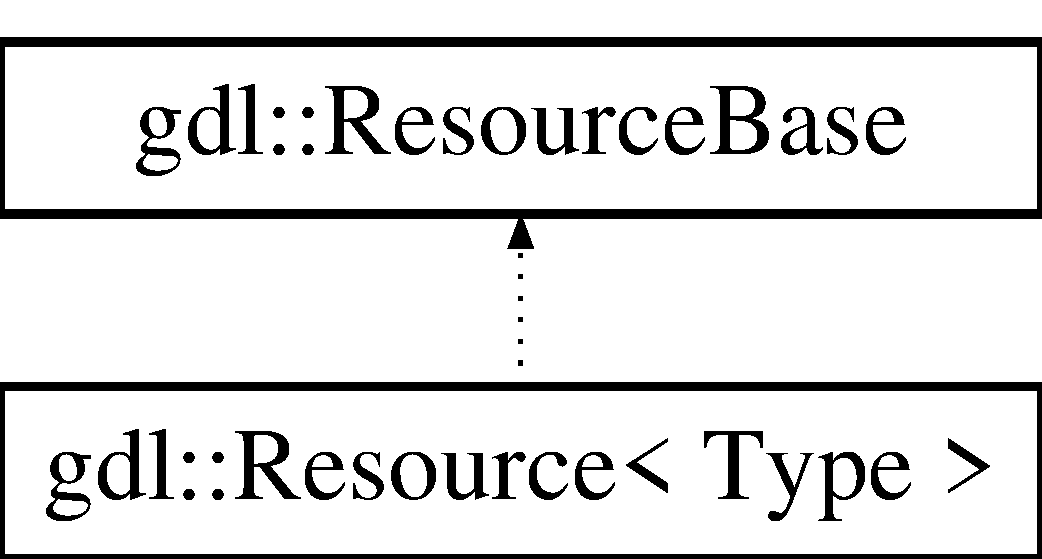
\includegraphics[height=2cm]{classgdl_1_1Resource}
\end{center}
\end{figure}
\subsection*{Public Member Functions}
\begin{DoxyCompactItemize}
\item 
\hyperlink{classgdl_1_1Resource_a149a477edeec7571d7664ac6be21f3ce}{Resource} (Type $\ast$val)
\item 
\hyperlink{classgdl_1_1Resource_a2110d7edf4e2864a70688a4279480e43}{Resource} (\hyperlink{classgdl_1_1Resource}{Resource} const \&)
\item 
\hyperlink{classgdl_1_1Resource}{Resource} \& \hyperlink{classgdl_1_1Resource_a8d4f9966f9a8047d0830fc0ce4c15d37}{operator=} (\hyperlink{classgdl_1_1Resource}{Resource} const \&)
\item 
virtual \hyperlink{classgdl_1_1Resource_a52f5853b3028356acb3cfe8673fa4bd3}{$\sim$Resource} ()
\item 
bool \hyperlink{classgdl_1_1Resource_a3d8b62b778b5c598ee51a5edcdae05ef}{isValid} () const 
\item 
Type $\ast$ \hyperlink{classgdl_1_1Resource_a0b869a1e27677c66bb78dec379e73658}{operator-\/$>$} ()
\item 
Type \& \hyperlink{classgdl_1_1Resource_a750113d7aafe245fecb39089d15ebbe3}{operator$\ast$} ()
\end{DoxyCompactItemize}
\subsection*{Protected Member Functions}
\begin{DoxyCompactItemize}
\item 
void \hyperlink{classgdl_1_1Resource_a62cfa0d7b8f63c2d6be09a644e49028c}{HardReset} ()
\end{DoxyCompactItemize}
\subsection*{Protected Attributes}
\begin{DoxyCompactItemize}
\item 
\hypertarget{classgdl_1_1Resource_acfc41dc044277eff21791ff867078989}{
Type $\ast$ {\bfseries data\_\-}}
\label{classgdl_1_1Resource_acfc41dc044277eff21791ff867078989}

\end{DoxyCompactItemize}
\subsubsection*{template$<$typename Type$>$ class gdl::Resource$<$ Type $>$}



\subsection{Constructor \& Destructor Documentation}
\hypertarget{classgdl_1_1Resource_a149a477edeec7571d7664ac6be21f3ce}{
\index{gdl::Resource@{gdl::Resource}!Resource@{Resource}}
\index{Resource@{Resource}!gdl::Resource@{gdl::Resource}}
\subsubsection[{Resource}]{\setlength{\rightskip}{0pt plus 5cm}template$<$typename Type$>$ {\bf gdl::Resource}$<$ Type $>$::{\bf Resource} (Type $\ast$ {\em val})\hspace{0.3cm}{\ttfamily  \mbox{[}inline, explicit\mbox{]}}}}
\label{classgdl_1_1Resource_a149a477edeec7571d7664ac6be21f3ce}
Explicit constructor.


\begin{DoxyParams}{Parameters}
\item[\mbox{$\leftarrow$} {\em val}]The pointer on a resource. \end{DoxyParams}
\hypertarget{classgdl_1_1Resource_a2110d7edf4e2864a70688a4279480e43}{
\index{gdl::Resource@{gdl::Resource}!Resource@{Resource}}
\index{Resource@{Resource}!gdl::Resource@{gdl::Resource}}
\subsubsection[{Resource}]{\setlength{\rightskip}{0pt plus 5cm}template$<$typename Type$>$ {\bf gdl::Resource}$<$ Type $>$::{\bf Resource} ({\bf Resource}$<$ Type $>$ const \& {\em right})\hspace{0.3cm}{\ttfamily  \mbox{[}inline\mbox{]}}}}
\label{classgdl_1_1Resource_a2110d7edf4e2864a70688a4279480e43}
Copy constructor.


\begin{DoxyParams}{Parameters}
\item[\mbox{$\leftarrow$} {\em right}]\hyperlink{classgdl_1_1Resource}{Resource} to copy. \end{DoxyParams}
\hypertarget{classgdl_1_1Resource_a52f5853b3028356acb3cfe8673fa4bd3}{
\index{gdl::Resource@{gdl::Resource}!$\sim$Resource@{$\sim$Resource}}
\index{$\sim$Resource@{$\sim$Resource}!gdl::Resource@{gdl::Resource}}
\subsubsection[{$\sim$Resource}]{\setlength{\rightskip}{0pt plus 5cm}template$<$typename Type $>$ {\bf gdl::Resource}$<$ Type $>$::$\sim${\bf Resource} ()\hspace{0.3cm}{\ttfamily  \mbox{[}inline, virtual\mbox{]}}}}
\label{classgdl_1_1Resource_a52f5853b3028356acb3cfe8673fa4bd3}
Default destructor. 

\subsection{Member Function Documentation}
\hypertarget{classgdl_1_1Resource_a62cfa0d7b8f63c2d6be09a644e49028c}{
\index{gdl::Resource@{gdl::Resource}!HardReset@{HardReset}}
\index{HardReset@{HardReset}!gdl::Resource@{gdl::Resource}}
\subsubsection[{HardReset}]{\setlength{\rightskip}{0pt plus 5cm}template$<$typename Type $>$ void {\bf gdl::Resource}$<$ Type $>$::HardReset ()\hspace{0.3cm}{\ttfamily  \mbox{[}inline, protected\mbox{]}}}}
\label{classgdl_1_1Resource_a62cfa0d7b8f63c2d6be09a644e49028c}
Reset the data. \hypertarget{classgdl_1_1Resource_a3d8b62b778b5c598ee51a5edcdae05ef}{
\index{gdl::Resource@{gdl::Resource}!isValid@{isValid}}
\index{isValid@{isValid}!gdl::Resource@{gdl::Resource}}
\subsubsection[{isValid}]{\setlength{\rightskip}{0pt plus 5cm}template$<$typename Type $>$ bool {\bf gdl::Resource}$<$ Type $>$::isValid () const\hspace{0.3cm}{\ttfamily  \mbox{[}inline\mbox{]}}}}
\label{classgdl_1_1Resource_a3d8b62b778b5c598ee51a5edcdae05ef}
Check if the resource is valid.

\begin{DoxyReturn}{Returns}
If valid, true is returned. Otherwise, false is returned. 
\end{DoxyReturn}
\hypertarget{classgdl_1_1Resource_a750113d7aafe245fecb39089d15ebbe3}{
\index{gdl::Resource@{gdl::Resource}!operator$\ast$@{operator$\ast$}}
\index{operator$\ast$@{operator$\ast$}!gdl::Resource@{gdl::Resource}}
\subsubsection[{operator$\ast$}]{\setlength{\rightskip}{0pt plus 5cm}template$<$typename Type $>$ Type \& {\bf gdl::Resource}$<$ Type $>$::operator$\ast$ ()\hspace{0.3cm}{\ttfamily  \mbox{[}inline\mbox{]}}}}
\label{classgdl_1_1Resource_a750113d7aafe245fecb39089d15ebbe3}
Overloading of the indirection operator. \hypertarget{classgdl_1_1Resource_a0b869a1e27677c66bb78dec379e73658}{
\index{gdl::Resource@{gdl::Resource}!operator-\/$>$@{operator-\/$>$}}
\index{operator-\/$>$@{operator-\/$>$}!gdl::Resource@{gdl::Resource}}
\subsubsection[{operator-\/$>$}]{\setlength{\rightskip}{0pt plus 5cm}template$<$typename Type $>$ Type $\ast$ {\bf gdl::Resource}$<$ Type $>$::operator-\/$>$ ()\hspace{0.3cm}{\ttfamily  \mbox{[}inline\mbox{]}}}}
\label{classgdl_1_1Resource_a0b869a1e27677c66bb78dec379e73658}
Overloading of the member operator. \hypertarget{classgdl_1_1Resource_a8d4f9966f9a8047d0830fc0ce4c15d37}{
\index{gdl::Resource@{gdl::Resource}!operator=@{operator=}}
\index{operator=@{operator=}!gdl::Resource@{gdl::Resource}}
\subsubsection[{operator=}]{\setlength{\rightskip}{0pt plus 5cm}template$<$typename Type $>$ {\bf gdl::Resource}$<$ Type $>$ \& {\bf gdl::Resource}$<$ Type $>$::operator= ({\bf Resource}$<$ Type $>$ const \& {\em right})\hspace{0.3cm}{\ttfamily  \mbox{[}inline\mbox{]}}}}
\label{classgdl_1_1Resource_a8d4f9966f9a8047d0830fc0ce4c15d37}
Overloading of the assignment operator.

\begin{DoxyReturn}{Returns}
An reference on the \hyperlink{classgdl_1_1Resource}{Resource} instance. 
\end{DoxyReturn}


The documentation for this class was generated from the following files:\begin{DoxyCompactItemize}
\item 
Resource.hpp\item 
Resource.inl\end{DoxyCompactItemize}

\hypertarget{classgdl_1_1ResourceBase}{
\section{gdl::ResourceBase Class Reference}
\label{classgdl_1_1ResourceBase}\index{gdl::ResourceBase@{gdl::ResourceBase}}
}
Inheritance diagram for gdl::ResourceBase::\begin{figure}[H]
\begin{center}
\leavevmode
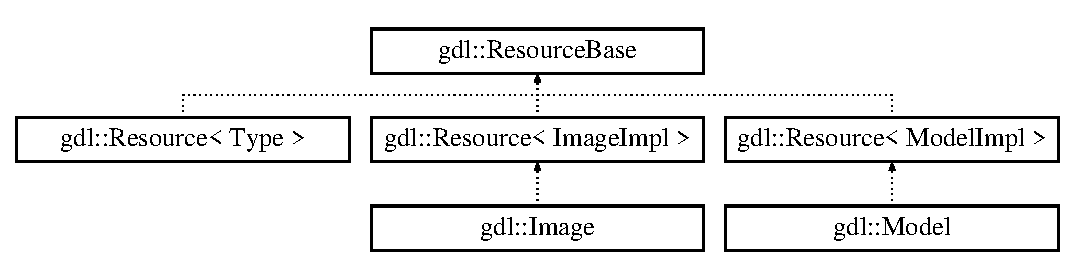
\includegraphics[height=3cm]{classgdl_1_1ResourceBase}
\end{center}
\end{figure}
\subsection*{Public Member Functions}
\begin{DoxyCompactItemize}
\item 
\hyperlink{classgdl_1_1ResourceBase_a0289636bcf3853381deb2325703d6d3d}{ResourceBase} ()
\item 
\hyperlink{classgdl_1_1ResourceBase_a8fc7453fe6219c010c42d31df1940e7e}{ResourceBase} (\hyperlink{classgdl_1_1ResourceBase}{ResourceBase} const \&right)
\item 
virtual \hyperlink{classgdl_1_1ResourceBase_afc2de70f0ca229deef3e5a5af1399736}{$\sim$ResourceBase} ()
\item 
\hyperlink{classgdl_1_1ResourceBase}{ResourceBase} \& \hyperlink{classgdl_1_1ResourceBase_a6655b5024b90d376ba4ed4f807d03f90}{operator=} (\hyperlink{classgdl_1_1ResourceBase}{ResourceBase} const \&)
\end{DoxyCompactItemize}
\subsection*{Protected Member Functions}
\begin{DoxyCompactItemize}
\item 
void \hyperlink{classgdl_1_1ResourceBase_add4498c5016ed85778964adc7b932412}{check\_\-destroy} ()
\end{DoxyCompactItemize}


\subsection{Constructor \& Destructor Documentation}
\hypertarget{classgdl_1_1ResourceBase_a0289636bcf3853381deb2325703d6d3d}{
\index{gdl::ResourceBase@{gdl::ResourceBase}!ResourceBase@{ResourceBase}}
\index{ResourceBase@{ResourceBase}!gdl::ResourceBase@{gdl::ResourceBase}}
\subsubsection[{ResourceBase}]{\setlength{\rightskip}{0pt plus 5cm}gdl::ResourceBase::ResourceBase ()}}
\label{classgdl_1_1ResourceBase_a0289636bcf3853381deb2325703d6d3d}
Default constructor. \hypertarget{classgdl_1_1ResourceBase_a8fc7453fe6219c010c42d31df1940e7e}{
\index{gdl::ResourceBase@{gdl::ResourceBase}!ResourceBase@{ResourceBase}}
\index{ResourceBase@{ResourceBase}!gdl::ResourceBase@{gdl::ResourceBase}}
\subsubsection[{ResourceBase}]{\setlength{\rightskip}{0pt plus 5cm}gdl::ResourceBase::ResourceBase ({\bf ResourceBase} const \& {\em right})}}
\label{classgdl_1_1ResourceBase_a8fc7453fe6219c010c42d31df1940e7e}
Copy constructor. \hypertarget{classgdl_1_1ResourceBase_afc2de70f0ca229deef3e5a5af1399736}{
\index{gdl::ResourceBase@{gdl::ResourceBase}!$\sim$ResourceBase@{$\sim$ResourceBase}}
\index{$\sim$ResourceBase@{$\sim$ResourceBase}!gdl::ResourceBase@{gdl::ResourceBase}}
\subsubsection[{$\sim$ResourceBase}]{\setlength{\rightskip}{0pt plus 5cm}virtual gdl::ResourceBase::$\sim$ResourceBase ()\hspace{0.3cm}{\ttfamily  \mbox{[}virtual\mbox{]}}}}
\label{classgdl_1_1ResourceBase_afc2de70f0ca229deef3e5a5af1399736}
Default destructor. 

\subsection{Member Function Documentation}
\hypertarget{classgdl_1_1ResourceBase_add4498c5016ed85778964adc7b932412}{
\index{gdl::ResourceBase@{gdl::ResourceBase}!check\_\-destroy@{check\_\-destroy}}
\index{check\_\-destroy@{check\_\-destroy}!gdl::ResourceBase@{gdl::ResourceBase}}
\subsubsection[{check\_\-destroy}]{\setlength{\rightskip}{0pt plus 5cm}void gdl::ResourceBase::check\_\-destroy ()\hspace{0.3cm}{\ttfamily  \mbox{[}protected\mbox{]}}}}
\label{classgdl_1_1ResourceBase_add4498c5016ed85778964adc7b932412}
Check if the data pointer can be destroyed. \hypertarget{classgdl_1_1ResourceBase_a6655b5024b90d376ba4ed4f807d03f90}{
\index{gdl::ResourceBase@{gdl::ResourceBase}!operator=@{operator=}}
\index{operator=@{operator=}!gdl::ResourceBase@{gdl::ResourceBase}}
\subsubsection[{operator=}]{\setlength{\rightskip}{0pt plus 5cm}{\bf ResourceBase}\& gdl::ResourceBase::operator= ({\bf ResourceBase} const \&)}}
\label{classgdl_1_1ResourceBase_a6655b5024b90d376ba4ed4f807d03f90}
Overloading of the assignment operator. 

The documentation for this class was generated from the following file:\begin{DoxyCompactItemize}
\item 
Resource.hpp\end{DoxyCompactItemize}

\hypertarget{classgdl_1_1Window}{
\section{gdl::Window Class Reference}
\label{classgdl_1_1Window}\index{gdl::Window@{gdl::Window}}
}


{\ttfamily \#include $<$Window.hpp$>$}\subsection*{Public Member Functions}
\begin{DoxyCompactItemize}
\item 
\hyperlink{classgdl_1_1Window_af775c74ba07b8ec16ed378b970406635}{Window} (void)
\item 
\hyperlink{classgdl_1_1Window_adf0d05debac3ac1bc05a75b171746c27}{$\sim$Window} (void)
\item 
void \hyperlink{classgdl_1_1Window_a616a4e27c611911476e5bfa3e85e915d}{create} (void)
\item 
void \hyperlink{classgdl_1_1Window_a9c9db9cf7e7a9d5b8b3ab98f24057582}{catchEvent} (void)
\item 
void \hyperlink{classgdl_1_1Window_ab58fa5ccc3a51ae3393465fcb04f5157}{display} (void)
\item 
void \hyperlink{classgdl_1_1Window_a72e440ef14e7e19754d4d7a548fd2f63}{close} (void)
\item 
bool \hyperlink{classgdl_1_1Window_a1d6572c0dde559d4f36608ddcc519e82}{isOpened} (void)
\item 
void \hyperlink{classgdl_1_1Window_a53e25fd5c288569ae28a01c56767a9c6}{setTitle} (std::string const \&title)
\item 
void \hyperlink{classgdl_1_1Window_a96e78a7ef90ba4f1166a282940f3990a}{setWidth} (size\_\-t const width)
\item 
void \hyperlink{classgdl_1_1Window_a1be26b215f0ac9b3f075616d53927646}{setHeight} (size\_\-t const height)
\item 
size\_\-t \hyperlink{classgdl_1_1Window_abe7946e48e470c1e4ef6ae56a83ae620}{getWidth} () const 
\item 
size\_\-t \hyperlink{classgdl_1_1Window_a9cb9feedb7ccdc129f9212448b4221b9}{getHeight} () const 
\item 
void \hyperlink{classgdl_1_1Window_a5834fddbeb60f10da3a7042f202e439c}{setFullscreen} (bool const state)
\item 
void \hyperlink{classgdl_1_1Window_a75799cef28dc31c7333f73409a1d712a}{setCursorAt} (unsigned int const x, unsigned int const y)
\item 
void \hyperlink{classgdl_1_1Window_afea7afeccaf67cc6f93a4690cebfe529}{showCursor} (bool const status)
\end{DoxyCompactItemize}
\subsection*{Friends}
\begin{DoxyCompactItemize}
\item 
class \hyperlink{classgdl_1_1Window_a4f546444e7f94a497ab5e72b5354f3af}{InputImpl}
\end{DoxyCompactItemize}


\subsection{Detailed Description}
The \hyperlink{classgdl_1_1Window}{Window} class offert you an OpenGL context. 

\subsection{Constructor \& Destructor Documentation}
\hypertarget{classgdl_1_1Window_af775c74ba07b8ec16ed378b970406635}{
\index{gdl::Window@{gdl::Window}!Window@{Window}}
\index{Window@{Window}!gdl::Window@{gdl::Window}}
\subsubsection[{Window}]{\setlength{\rightskip}{0pt plus 5cm}gdl::Window::Window (void)}}
\label{classgdl_1_1Window_af775c74ba07b8ec16ed378b970406635}
Construct \hyperlink{classgdl_1_1Window}{Window} object with default values.\par
 Title : \char`\"{}Game\char`\"{}\par
 Width : 800\par
 Height : 600\par
 Fullscreen mode : false\par
 \hypertarget{classgdl_1_1Window_adf0d05debac3ac1bc05a75b171746c27}{
\index{gdl::Window@{gdl::Window}!$\sim$Window@{$\sim$Window}}
\index{$\sim$Window@{$\sim$Window}!gdl::Window@{gdl::Window}}
\subsubsection[{$\sim$Window}]{\setlength{\rightskip}{0pt plus 5cm}gdl::Window::$\sim$Window (void)}}
\label{classgdl_1_1Window_adf0d05debac3ac1bc05a75b171746c27}
Destroy \hyperlink{classgdl_1_1Window}{Window} object. 

\subsection{Member Function Documentation}
\hypertarget{classgdl_1_1Window_a9c9db9cf7e7a9d5b8b3ab98f24057582}{
\index{gdl::Window@{gdl::Window}!catchEvent@{catchEvent}}
\index{catchEvent@{catchEvent}!gdl::Window@{gdl::Window}}
\subsubsection[{catchEvent}]{\setlength{\rightskip}{0pt plus 5cm}void gdl::Window::catchEvent (void)}}
\label{classgdl_1_1Window_a9c9db9cf7e7a9d5b8b3ab98f24057582}
Catch the event when the user closes the window. \hypertarget{classgdl_1_1Window_a72e440ef14e7e19754d4d7a548fd2f63}{
\index{gdl::Window@{gdl::Window}!close@{close}}
\index{close@{close}!gdl::Window@{gdl::Window}}
\subsubsection[{close}]{\setlength{\rightskip}{0pt plus 5cm}void gdl::Window::close (void)}}
\label{classgdl_1_1Window_a72e440ef14e7e19754d4d7a548fd2f63}
Close the window \hypertarget{classgdl_1_1Window_a616a4e27c611911476e5bfa3e85e915d}{
\index{gdl::Window@{gdl::Window}!create@{create}}
\index{create@{create}!gdl::Window@{gdl::Window}}
\subsubsection[{create}]{\setlength{\rightskip}{0pt plus 5cm}void gdl::Window::create (void)}}
\label{classgdl_1_1Window_a616a4e27c611911476e5bfa3e85e915d}
Create (or recreate) the \hyperlink{classgdl_1_1Window}{Window}. \hypertarget{classgdl_1_1Window_ab58fa5ccc3a51ae3393465fcb04f5157}{
\index{gdl::Window@{gdl::Window}!display@{display}}
\index{display@{display}!gdl::Window@{gdl::Window}}
\subsubsection[{display}]{\setlength{\rightskip}{0pt plus 5cm}void gdl::Window::display (void)}}
\label{classgdl_1_1Window_ab58fa5ccc3a51ae3393465fcb04f5157}
Display the window on screen. \hypertarget{classgdl_1_1Window_a9cb9feedb7ccdc129f9212448b4221b9}{
\index{gdl::Window@{gdl::Window}!getHeight@{getHeight}}
\index{getHeight@{getHeight}!gdl::Window@{gdl::Window}}
\subsubsection[{getHeight}]{\setlength{\rightskip}{0pt plus 5cm}size\_\-t gdl::Window::getHeight (void) const}}
\label{classgdl_1_1Window_a9cb9feedb7ccdc129f9212448b4221b9}
Get the Windows's Height \hypertarget{classgdl_1_1Window_abe7946e48e470c1e4ef6ae56a83ae620}{
\index{gdl::Window@{gdl::Window}!getWidth@{getWidth}}
\index{getWidth@{getWidth}!gdl::Window@{gdl::Window}}
\subsubsection[{getWidth}]{\setlength{\rightskip}{0pt plus 5cm}size\_\-t gdl::Window::getWidth (void) const}}
\label{classgdl_1_1Window_abe7946e48e470c1e4ef6ae56a83ae620}
Get the Windows's Width \hypertarget{classgdl_1_1Window_a1d6572c0dde559d4f36608ddcc519e82}{
\index{gdl::Window@{gdl::Window}!isOpened@{isOpened}}
\index{isOpened@{isOpened}!gdl::Window@{gdl::Window}}
\subsubsection[{isOpened}]{\setlength{\rightskip}{0pt plus 5cm}bool gdl::Window::isOpened (void)}}
\label{classgdl_1_1Window_a1d6572c0dde559d4f36608ddcc519e82}
Tell if the window is open.

\begin{DoxyReturn}{Returns}
If the window is open, true is returned. Otherwise, false is returned. 
\end{DoxyReturn}
\hypertarget{classgdl_1_1Window_a75799cef28dc31c7333f73409a1d712a}{
\index{gdl::Window@{gdl::Window}!setCursorAt@{setCursorAt}}
\index{setCursorAt@{setCursorAt}!gdl::Window@{gdl::Window}}
\subsubsection[{setCursorAt}]{\setlength{\rightskip}{0pt plus 5cm}void gdl::Window::setCursorAt (unsigned int const  {\em x}, \/  unsigned int const  {\em y})}}
\label{classgdl_1_1Window_a75799cef28dc31c7333f73409a1d712a}
Set the cursor at a specified position.


\begin{DoxyParams}{Parameters}
\item[\mbox{$\leftarrow$} {\em x}]Position on x-\/axis (from left) \item[\mbox{$\leftarrow$} {\em y}]Position on y-\/axis (from top) \end{DoxyParams}
\hypertarget{classgdl_1_1Window_a5834fddbeb60f10da3a7042f202e439c}{
\index{gdl::Window@{gdl::Window}!setFullscreen@{setFullscreen}}
\index{setFullscreen@{setFullscreen}!gdl::Window@{gdl::Window}}
\subsubsection[{setFullscreen}]{\setlength{\rightskip}{0pt plus 5cm}void gdl::Window::setFullscreen (bool const  {\em state})}}
\label{classgdl_1_1Window_a5834fddbeb60f10da3a7042f202e439c}
Set the fullscreen mode to the window.


\begin{DoxyParams}{Parameters}
\item[\mbox{$\leftarrow$} {\em state}]True to set the fullscreen mode. False to set windowed mode. \end{DoxyParams}
\hypertarget{classgdl_1_1Window_a1be26b215f0ac9b3f075616d53927646}{
\index{gdl::Window@{gdl::Window}!setHeight@{setHeight}}
\index{setHeight@{setHeight}!gdl::Window@{gdl::Window}}
\subsubsection[{setHeight}]{\setlength{\rightskip}{0pt plus 5cm}void gdl::Window::setHeight (size\_\-t const  {\em height})}}
\label{classgdl_1_1Window_a1be26b215f0ac9b3f075616d53927646}
Set the height to the window. Must be called before create method.


\begin{DoxyParams}{Parameters}
\item[{\em height}]New height. \end{DoxyParams}
\hypertarget{classgdl_1_1Window_a53e25fd5c288569ae28a01c56767a9c6}{
\index{gdl::Window@{gdl::Window}!setTitle@{setTitle}}
\index{setTitle@{setTitle}!gdl::Window@{gdl::Window}}
\subsubsection[{setTitle}]{\setlength{\rightskip}{0pt plus 5cm}void gdl::Window::setTitle (std::string const \& {\em title})}}
\label{classgdl_1_1Window_a53e25fd5c288569ae28a01c56767a9c6}
Set the title to the window. Must be called before create method.


\begin{DoxyParams}{Parameters}
\item[\mbox{$\leftarrow$} {\em title}]New title. \end{DoxyParams}
\hypertarget{classgdl_1_1Window_a96e78a7ef90ba4f1166a282940f3990a}{
\index{gdl::Window@{gdl::Window}!setWidth@{setWidth}}
\index{setWidth@{setWidth}!gdl::Window@{gdl::Window}}
\subsubsection[{setWidth}]{\setlength{\rightskip}{0pt plus 5cm}void gdl::Window::setWidth (size\_\-t const  {\em width})}}
\label{classgdl_1_1Window_a96e78a7ef90ba4f1166a282940f3990a}
Set the width to the window. Must be called before create method.


\begin{DoxyParams}{Parameters}
\item[\mbox{$\leftarrow$} {\em width}]New width. \end{DoxyParams}
\hypertarget{classgdl_1_1Window_afea7afeccaf67cc6f93a4690cebfe529}{
\index{gdl::Window@{gdl::Window}!showCursor@{showCursor}}
\index{showCursor@{showCursor}!gdl::Window@{gdl::Window}}
\subsubsection[{showCursor}]{\setlength{\rightskip}{0pt plus 5cm}void gdl::Window::showCursor (bool const  {\em status})}}
\label{classgdl_1_1Window_afea7afeccaf67cc6f93a4690cebfe529}
Show or hide the mouse cursor.


\begin{DoxyParams}{Parameters}
\item[\mbox{$\leftarrow$} {\em status}]True to show the cursor. False to hide it. \end{DoxyParams}


\subsection{Friends And Related Function Documentation}
\hypertarget{classgdl_1_1Window_a4f546444e7f94a497ab5e72b5354f3af}{
\index{gdl::Window@{gdl::Window}!InputImpl@{InputImpl}}
\index{InputImpl@{InputImpl}!gdl::Window@{gdl::Window}}
\subsubsection[{InputImpl}]{\setlength{\rightskip}{0pt plus 5cm}friend class InputImpl\hspace{0.3cm}{\ttfamily  \mbox{[}friend\mbox{]}}}}
\label{classgdl_1_1Window_a4f546444e7f94a497ab5e72b5354f3af}
To reach private members of InputImpl. 

The documentation for this class was generated from the following files:\begin{DoxyCompactItemize}
\item 
Window.hpp\item 
Window.cpp\end{DoxyCompactItemize}

\printindex
\end{document}
